\documentclass[a4paper,DIV12]{scrartcl}
\usepackage{graphicx}
\usepackage{natbib}
\usepackage{amsmath}
\usepackage{comment}
\usepackage{url}
\usepackage{color}
\usepackage{listings}
\usepackage[pdftex]{hyperref}
\graphicspath{{pics/}}
\DeclareMathOperator{\diag}{diag}
\DeclareMathOperator{\IRLS}{IRLS}
%matrices
\newcommand{\A}{\mathbf{A}}
\newcommand{\B}{{\bf B}}
\newcommand{\C}{\mathbf{C}} % constraint matrix, alt. \W_m
\newcommand{\Cd}{\mathbf{C_d}} % data covariance, alt. \W_m
\newcommand{\Cm}{\mathbf{C_m}} % data covariance, alt. \W_m
\newcommand{\D}{\mathbf{D}} % data weighting matrix, alt. \W_d
\newcommand{\F}{\mathbf{F}} % forward matrix for linear case
\renewcommand{\H}{\mathbf{H}} % Hessian
\newcommand{\I}{\mathbf{I}} % identity
\renewcommand{\P}{\mathbf{P}} % parameter matrix
\newcommand{\R}{{\bf R}} % resolution matrix
\renewcommand{\S}{\mathbf{S}} % Sensitivity matrix
\newcommand{\SV}{\mathbf{\Lambda}} % Singul�rwertmatrix , alt. \Sigma
\renewcommand{\SS}{\mathbf{\widehat{S}}} % data-scaled Sensitivity
\newcommand{\U}{\mathbf{U}} % Datenvektoren, alt. \V_D
\newcommand{\V}{\mathbf{V}} % Modellvektoren, alt. \V_M
\newcommand{\W}{\mathbf{W}}
\newcommand{\Null}{\mathbf{0}} % the null matrix
%vectors
\renewcommand{\b}{\mathbf{b}}
\renewcommand{\c}{\mathbf{c}}
\renewcommand{\d}{\mathbf{d}}
\newcommand{\f}{\mathbf{f}}
\newcommand{\g}{\mathbf{g}}
\newcommand{\m}{\mathbf{m}}
\newcommand{\n}{\mathbf{n}}
\renewcommand{\j}{\mathbf{j}}
\newcommand{\p}{\mathbf{p}}
\newcommand{\q}{\mathbf{q}}
\renewcommand{\r}{\mathbf{r}}
\renewcommand{\u}{\mathbf{u}}
\renewcommand{\v}{\mathbf{v}}
\newcommand{\tv}{\mathbf{\tilde v}}
\newcommand{\w}{\mathbf{w}}
\newcommand{\x}{\mathbf{x}}
\newcommand{\y}{\mathbf{y}}
\newcommand{\z}{\mathbf{z}}
%vector components
\newcommand{\ui}{\mathbf{u_i}}
\newcommand{\vi}{\mathbf{v_i}}
\newcommand{\wi}{\mathbf{w_i}}
% still unfixed denotations
\newcommand{\stdev}{\sigma}
\newcommand{\proz}{\varepsilon}
\newcommand{\gphi}{\mathbf{g}} % simple gradient
\newcommand{\err}{\epsilon} % error
\newcommand{\potvec}{\boldsymbol{\varphi}} % 
\newcommand{\nd}{N} % number of data, alt. n_d, d
\newcommand{\nm}{M} % number of model parameter, alt. n_m, m
\renewcommand{\ne}{E} % number of electrodes, alt. n_e, e
\newcommand{\sig}{\sigma}
\newcommand{\bsig}{{\bf\sig}}
\newcommand{\Sig}{\mathbf{\Sigma}}
\newcommand{\K}{\mathbf{K}}
% constructs
\newcommand{\Cov}{\mbox{Cov}}
%\newcommand{\Cov}{\mbox{MCM}}
\newcommand{\norm}[1]{\left\| #1 \right\|} 
\newcommand{\gradm}{{\bf\nabla_m}} % model-nabla vector
\newcommand{\gradmq}{{\bf\nabla^2_m}} % model-nabla vector
\newcommand{\mgphi}{{\bf\gamma}} % negative gradient (cg)
%\newcommand{\diag}[1]{\mbox{diag}(#1)}
\newcommand{\Diag}[1]{\mbox{diag}\left(#1\right)}
\newcommand{\dd}[2]{\frac{\partial #1}{\partial #2}}
\newcommand{\dint}{\,\operatorname{d}\!} % integration d   
\newcommand{\dqd}[3]{\frac{\partial^2 #1}{\partial #2 \partial #3}}
\newcommand{\inR}[1]{\in\mathbb{R}^{#1}} % fehlendes \mathbb
\newcommand{\comm}[1]{\quad\mbox{#1}\quad}
\newcommand{\pu}[2]{$#1\,$#2} % value physical unit
\newcommand{\ppu}[3]{$#1\!-\!#2\,$#3} % value physical unit
\newcommand{\xpu}[3]{$#1\!=\!#2\,$#3} % value physical unit
\newcommand{\xppu}[4]{$#1\!=\!#2\!-\!#3\,$#4} % value physical unit
\newcommand{\ohmm}{\mbox{$\Omega\,$m}}
\newcommand{\om}[1]{\pu{#1}{\ohmm}} % Ohmmeters
%\newcommand{\inR}[1]{\in R^{#1}}
% DC resistivity stuff
\newcommand{\AM}{\overline{AM}}
\newcommand{\AN}{\overline{AN}}
\newcommand{\BM}{\overline{BM}}
\newcommand{\BN}{\overline{BN}}
\newcommand{\AsM}{\overline{A'M}}
\newcommand{\AsN}{\overline{A'N}}
\newcommand{\BsM}{\overline{B'M}}
\newcommand{\BsN}{\overline{B'N}}
\newcommand{\kq}{\overline{k}}
% layout things
%\newcommand{\sssec}[1]{\minipage{#1}}
%\newcommand{\sssec}[1]{\subsubsection{#1}}
\newcommand{\sssec}[1]{\subsubsection*{#1}}
\newcommand{\half}{0.48\columnwidth}
\newcommand{\third}{0.32\columnwidth}
\newcommand{\halfpic}{0.48\textwidth}
\newcommand{\plainpage}[2]{
\def\abstractname{#1} \begin{abstract} \input #2 \end{abstract}} 
\newcommand{\abstr}[2]{
\clearpage\thispagestyle{empty}\subsection*{#1}\input #2}
%\newcommand{\app}[1]{
%\begin{appendix}
%\addcontentsline{toc}{section}{#1}
%\section*{#1}
%\end{appendix}}

\bibliographystyle{apalike}
\parindent 0pt
\author{
Thomas G{\"u}nther\thanks{Leibniz Institute for Applied Geophysics, Hannover (Germany)} 
\ \& \ 
Carsten R{\"u}cker\thanks{Institute of Geology and Geophysics, University of Leipzig (Germany)}
}
\title{GIMLi --\\ Geophysical Inversion and Modelling Library \\-- programmers tutorial}
\newcommand{\cw}[1]{{\textbf{\texttt{#1}}}}
\newcommand{\invert}{invert}
\newcommand{\command}[1]{\par{\texttt{\$ #1}}}
\newcommand{\file}[1]{{\texttt{#1}}}
\newcommand{\sperre}{\,\rule{1ex}{2ex}}
\newcommand{\mycomment}[2]{\sperre{\textem{#1: #2}}\sperre}

\lstloadlanguages{[Visual]C++,[ISO]C++,Python}
\lstset{language=[ISO]C++}
\lstdefinelanguage{C++}{morekeywords={RVector,RMatrix,ModellingBase}}
%\lstset{numbers=left,numberstyle=\tiny}
%\lstset{basicstyle=\small,keywordstyle=\color{red}}
\lstset{basicstyle=\sffamily\small,keywordstyle=\bfseries}
\lstset{frame=shadowbox,commentstyle=\color{blue}}
\lstset{morekeywords={RVector,RMatrix,ModellingBase,RSparseMapMatrix,SparseMatrix}}

\begin{document}
\maketitle
\begin{abstract}
GIMLi is a C++ class library for solving inverse and forward problems in geophysics.
It was build in order to make inversion available to various forward modelling routines.
Template programming algorithms are used to create a purely mathematical framework for solving physics problems.
The inversion can apply various minimisation and regularization schemes, different transformation functions a region approach for sophisticated regularization and the chance to incorporate parametric and structural inversion.

In this tutorial we like to show the programmer how to work with GIMLi by means of different examples.
A simple curve-fitting is used to show how different forward operators can be incorporated.
Some small 1d examples demonstrate the use of different parameterization and the partitioning of data and model.
The region technique can be used for different target parameters or geological units.

Joining different inversion runs is one of the key issues of ongoing research.
We show three different joint inversion (JI) types: one-parameter JI, petrophysical JI and structural JI.
Finally the time-lapse inversion framework is presented and applied to ERT data using different algorithms.
\end{abstract}

\clearpage
\tableofcontents

%%%%%%%%%%%%%%%%%%%%%%%%%%%%%%%%%%%%%%%%%%%%%%%%%%%
\section{Introduction}\label{sec:intro}
\subsection{GIMLi -- concept and overview}\label{sec:gimli}
In geophysics, various physical processes and fields are used to gain information about the subsurface parameters.
The fields and processes can be very well studied and understood by simulation assuming a parameter distribution.
This so-called forward task can be done by using analytical formulae and numerical integration, or numerical schemes deploying finite difference or finite element techniques.
In the recent years, very different studies have been presented that open up new methods to be used.

However, in almost all approaches the task is finally to derive subsurface parameters, i.e. the inverse problem has to be solved.
Very often this is ill-posed, i.e. a variety of solutions is fitting the data within error bounds.
Hence regularization methods have to be applied.
There exist numerous inversion and regularization schemes, which do not have to be reinvented.
Furthermore, often a resolution analysis is required in order to appraise the quality of the results.
The idea of GIMLi is to present a very flexible framework for geophysical inversion and modelling such that it can be used from any forward operator.
All problems such as optimization of regularization parameters, line search are solved generally.
The GIMLi library is structured into four layers (Fig.~\ref{fig:gimliblock}) that are based on each other:

\begin{description}
	\item[The basic layer] holds fundamental algebraic methods and mesh containers for model parameterisation 
	\item[The modelling\&region layer] administrates the modelling classes that are based on a basis class and the connection to constraints and transform functions
	\item[The inversion layer] is a template class for minimisation with different methods, inverse solvers, line search, $\lambda$ optimisation and resolution analysis
	\item[In Inversion frameworks] sophisticated techniques are formulated, e.g. time-lapse strategies, roll-along inversion or different kinds of joint inversion
\end{description}

\begin{figure}[htb]
\centering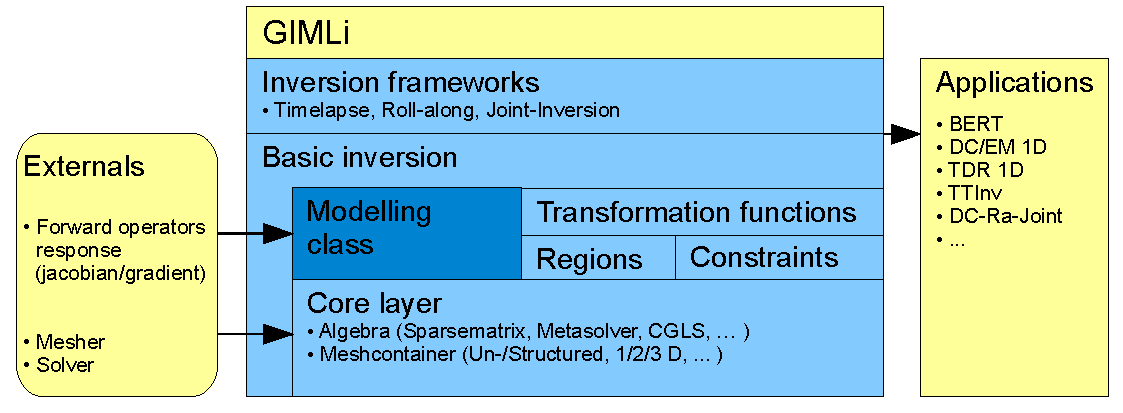
\includegraphics[width=0.85\textwidth]{gimliblock}
\caption{Scheme of the GIMLi library, applications and externals}\label{fig:gimliblock}
\end{figure} 

External programs are, e.g., mesh generators and solvers for linear systems.
For generating quality constrained irregular 2d and 3d meshes, we usually use \cw{Triangle}~\citep{triangle} and \cw{TetGen}~\citep{tetgen}.
For solving linear systems we recommend the open-source collection \cw{SuiteSparse} \citep{davis}, which contains multi-frontal direct\&iterative solvers as well as reordering algorithms.

External forward operators can be easily linked against GIMLi.
As soon they meet the requirements, the inversion can be setup and run with 2 lines.

%%%%%%%%%%%%%%%%%%%%%%%%%%%%%%%%%%%%%%%%%%%%%%%%%%%%%%%%%%%%%%%%%%%%%%%%%%%
\subsection{Minimisation and regularization methods}\label{sec:mini}
Assume we have a discrete number of data $d_i$ assembled in a data vector $\d=[d_1,\ldots,d_D]^T$.
We want to find a parameter distribution represented by a discrete model vector $\m=[m_1,\ldots,m_M]^T$ such that the forwad response $\f(\m)$ approximates $\d$.
To each datum a variance $\delta d_i$ is associated.
By weighting the individual misfit $f_i-d_i$ with $\delta d_i$ we obtain a unit-less misfit vector, such that different data are combined easily.

We try to minimise the misfit vector in a least squares sense using the objective function
\begin{equation}\label{eq:phid}
\Phi_d=\sum\limits_{i=1}{D} \left| \frac{d_i-f_i(\m)}{\delta d_i} \right|^2
= \big\Vert \D(\d - \f(\m)) \big\Vert^2_2 \rightarrow \min
\quad\mbox{with}\quad \D=\mbox{diag}(\delta d_i^{-1})\quad.
\end{equation}

More generally, the inverse data covariance matrix $\W_d^{-1}$ can be used instead of $\D$ if the variances are correlated.
Since the problem is usually non-unique, regularization has to be applied.
We concentrate on explicit and global regularization (CITE) and use a generalized matrix formulation (CITE) to obtain a model objective function 
\begin{equation}\label{eq:phim}
\Phi_m = \|\W^c \C \W^m (\m-\m^R)\|^2_2\quad.
\end{equation}

$\m^R$ represents a reference model.
The matrix $\C$ is a derivative matrix or an identity matrix or a mixture of it.
In the first neighboring relations are taken into account (smoothness constraints), whereas in the latter (zeroth order smoothness) they are not.
The assumption of a smooth model is often the only choice to cope with ill-posedness and limited resolution.
However the degree of smoothness can be controlled flexibly with the mostly diagonal weighting matrices $\W^b=\diag(w^b_i)$ and $\W^m=\diag(w^m_i)$.
A derivative matrix consists of $C$ rows or constraint equations constraining the $M$ model cells corresponding to the rows.
By choosing the $w^m_i$  each model cell can be weighted individually such that a varying degree of smoothness or vicinity to the reference model can be achieved. 
Doing so, parameter constraints are applied using cell-dependent regularization.
On the contrary, we are able to incorporate structural constraints by setting the the weights $w^c_i$ for the individual model boundaries. 
For example, we can allow for arbitrary contrasts along a known boundary (e.g. from seismics or boreholes) in an otherwise smooth model (CITE).

Finally, a regularization parameter $\lambda$ is used to weight $\Phi_d$ and $\Phi_m$ so that we minimize
\begin{equation}\label{eq:min}
\Phi = \Phi_d + \lambda\Phi_m = \big\Vert \D(\d - \f(\m)) \big\Vert^2_2 
+ \lambda \big\Vert\W^c \C \W^m (\m-\m^R)\big\Vert^2_2 \rightarrow \min\quad.
\end{equation}

Although the $w_i$ are already regularization parameters it is easier to use relative $w_i$ and optimized only the one external $\lambda$.
In the knowledge of the variances, $\lambda$ has to be chosen such that the data are fitted within their variances in a least squares sense. The inversion task can then be posed as
\[ \min\limits_{\m} \Phi_m \quad\mbox{subject to}\quad \chi^2=\Phi_d/N=1 \quad, \]
which yields the same result as equation \ref{eq:min} for appropriate $\lambda$.

There are different methods for minimisation.
The most popular one is a Gauss-Newton scheme since it has a fast convergence.
However it requires the computation of the jacobian or sensitivity matrix with the elements $J_{ij}=\frac{\partial f_i(\m)}{\partial m_j}$.
Some physical problems allow for efficient sensitivity approximation.
For small-scaled problems with fast forward operators it can be approximated by (brute force) variation of the $m_j$ and a forward calculation.

In Gauss-Newton inversion, a big equation system consisting of the matrices above is solved for the model update.
However, the left-hand side is not built up. 
Instead the equation is solved by conjugate-gradient based solvers that incorporate all matrices and vectors.

Alternative methods that do not need the storage of the are gradient-based.
The gradient 
\[ \g(\m) = \left[ \dd{\Phi}{m_1}, \dd{\Phi}{m_2}, \ldots \dd{\Phi}{m_M} \right]^T \]
splits up in the model gradient and data gradient.
The latter can be computed for some methods using adjoint field methods.
Otherwise it can be computed by the perturbation method as well.

The easiest method is the steepest descent method where the model update is sought in the negative gradient.
A more sophisticated and faster converging method is called nonlinear conjugate gradients (NLCG), where the preceding gradients are taken into account.
A hybrid method between gradient and Gauss-Newton method is the quasi-Newton method.
It successively stores the projections of the gradient directions and approximates the jacobian step-wise.
Thus it starts with the linear convergence of gradient methods but ends up with quadratic Gauss-Newton convergence without storage of the jacobian matrix.
This method is particularly interesting for higher-dimensional problems \citep{haber05}.

For all methods, an update $\Delta\m^{k+1}$ of the current model $\m^k$ is obtained.
The model is updated using a step length  $\tau^{k+1}$ such that equation~\ref{eq:min} is minimized.
The latter is called line search and can be done exact, by interpolation of the $f_i(\m^k+\Delta\m^{k+1})$ or by forward calculation of three step lengths and fitting a parabola.

%%%%%%%%%%%%%%%%%%%%%%%%%%%%%%%%%%%%%%%%%%%%%%%%%%%%%%%%%%%%%%%%%%%%%%%%%%%
\subsubsection*{Forward operator requirement}\label{sec:forward}
A forward operator is defined by a C++ class object derived from a base forward operator class \cw{ModellingBase}.
The only necessary function is called \cw{response}, and it returns a forward response vector for a given model vector.
Once an instance f of class has been defined, the forward response for the model vector model is called by f.response( model ) or, more briefly, f( model ).

%%%%%%%%%%%%%%%%%%%%%%%%%%%%%%%%%%%%%%%%%%%%%%%%%%%%%%%%%%%%%%%%%%%%%%%%%%%
\subsection{Transformation functions}\label{sec:introtrans}
The forward problem is usually posed based on some intrinsic properties and measurements, e.g. the measured voltage is based on  conductivity.
However, we often want to use $d$ and $m$ values different from that, e.g. apparent resistivity and logarithm of resistivity.
Motivation for that may be a better-posed system, additional constraints such as positivity or the incorporation of petrophysical constraints \citep{tarantola01,guerue08nearsurface}.

In any GIMLi application we can choose arbitrary transformation functions in any stage of the inversion.
The inversion itself is using template classes such that the transformations are carried out on the fly.
The choice affects model and data vector, but also data weighting and of course the gradient and jacobian.
However the jacobian or gradient of the transformed inverse problem are never explicit formed, instead they are incorporated into the inverse sub-problem by using derivatives.

A transformation $\hat m(m)$ needs three things: the transformation from $m$ to $\hat m$ and back, and the derivative of $\hat m$ with respect to $m$. A number of useful transformation is already available. Others can be easily created or derived by combination of existing ones. See appendix \ref{app:trans} for details.

%%%%%%%%%%%%%%%%%%%%%%%%%%%%%%%%%%%%%%%%%%%%%%%%%%%%%%%%%%%%%%%%%%%%%%%%%%%
\subsection{Parameterisation and the region technique}\label{sec:parameter}
The discrete model parameters $m_i$ can be freely defined (without spatial association - 0d) or be coefficients for a given model parameterisation (1d, 2d, 3d or 4d) or a mixture of it.
A spatial parameterisaton is represented by a mesh containing the neighboring relations.
Figure~\ref{fig:para} shows different basic parameterisations.
This can be structured (e.g. a finite difference discretisaton) or unstructured arranged by triangles or tetrahedra.
There are various functions for mesh generation, export and import, see appendix~\ref{app:meshes}.

\begin{figure}[htbp]
\centering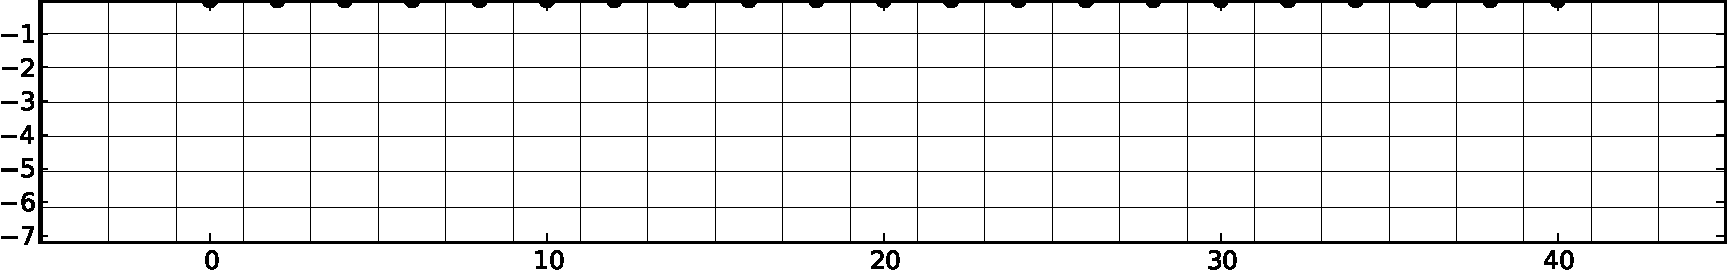
\includegraphics[width=0.45\textwidth]{structured2DMesh.pdf}\\
\centering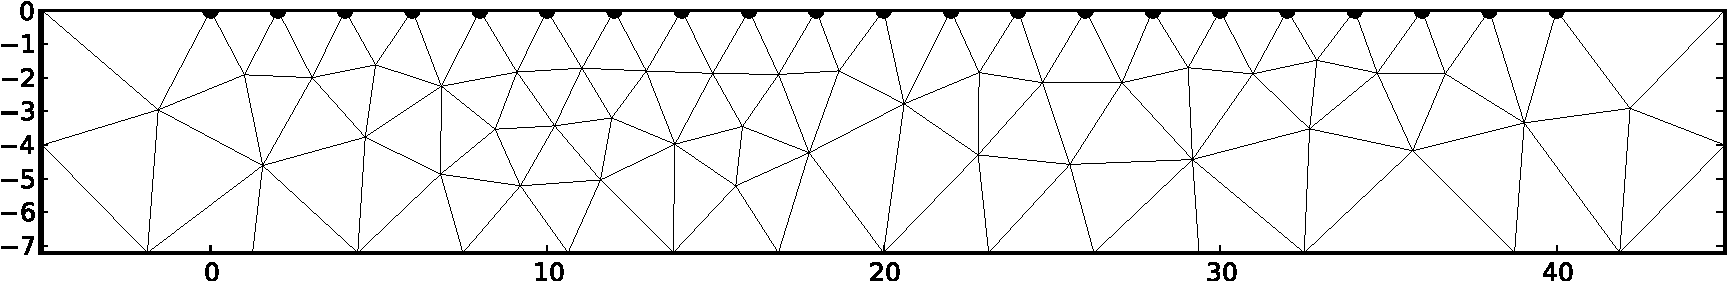
\includegraphics[width=0.45\textwidth]{unstructured2DMesh.pdf}\\
\centering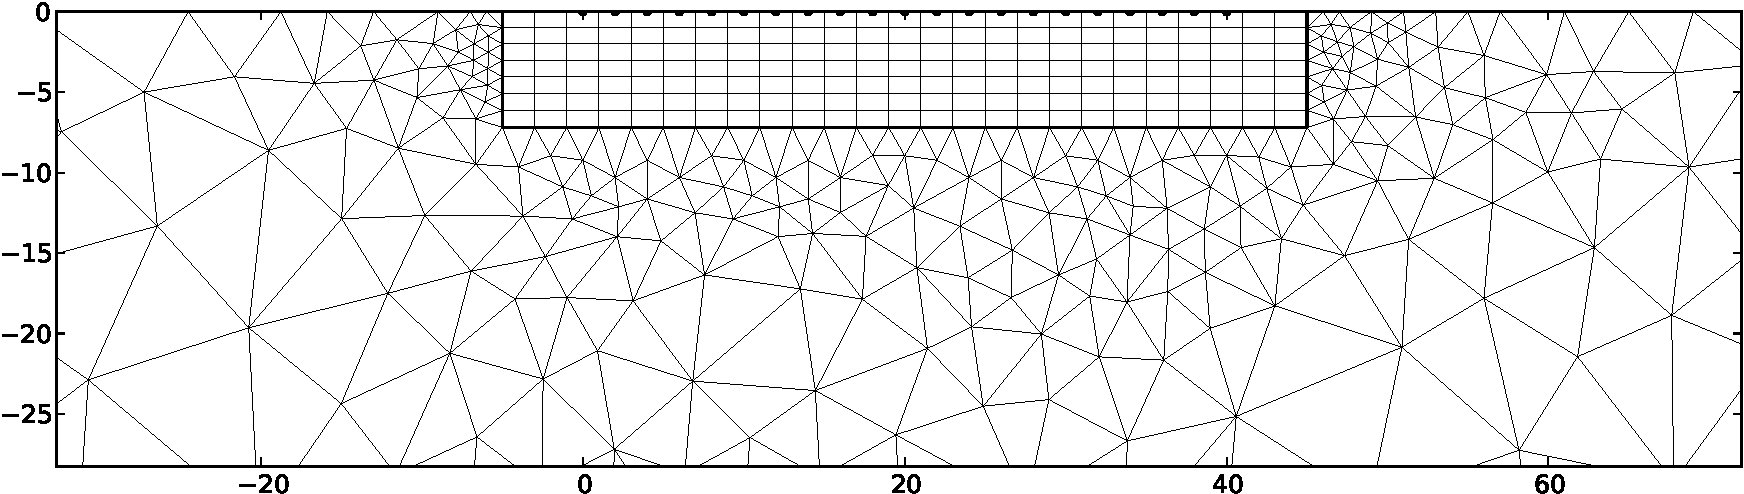
\includegraphics[width=0.45\textwidth]{mixed2DMesh.pdf}
\caption{Different parameterisations: 0d (independent parameters), 1d mesh, 2d structured mesh (grid), 2d unstructured mesh, 2d mixed mesh, 3d mesh}\label{fig:para}
\end{figure}

A combination of different data is easily achieved by the described error weighting and combining two vectors, e.g. amplitude and phase data in MT, in one vector.
Different parameters, can similarly be treated by different parts of the model vector, so-called regions.
Regions can be, as the name states, parts of one mesh representing different geological units.
Regions can also be different parameters on the same mesh (e.g. porosity and saturation) or on different parametrisations, e.g. a 2d/3d resistivity distribution and (0d) values for static shift in MT inversion.

In inversion the regions are by default independent from each other, but can as well be constrained to another.
For each region the starting model value, but also constraint type, model and constraint control and the used transformation function can be freely defined.
Special regions are a background region (not part of inversion) and a single-parameter region (all cells a compounded to one parameter). See appendix \ref{app:regions} for how to control the behaviour of regions.

%%%%%%%%%%%%%%%%%%%%%%%%%%%%%%%%%%%%%%%%%%%%%%%%%%%%%%%%%%%%%%%%%%%%%%%%%%%
\subsection{Obtaining and building GIMLi}
Since summer 2011, GIMLi is hosted on SourceForge under the project name libgimli\footnote{Note that since this change the BERT components were excluded from the project to a dedicated repository.}.
See \url{http://sourceforge.net/projects/libgimli/} for additional information such as binary downloads, documentation, bug tracker and feature request.
The code itself can be retrieved using subversion (SVN) using the address \url{https://libgimli.svn.sourceforge.net/svnroot/libgimli}.
As usual the code contains a current development (trunk), experimental changes or side-projects (branches) and stable versions (tags).

The main code is located under \file{src} and applications in different sub-folders under \file{apps}.
Under \file{doc} you will find Doxygen documentation and this tutorial including its code examples.
To build the binaries, the GNU build system (Autotools) is used: first, the script \cw{autogen.sh} runs the autotools and start the configuration \cw{configure} and \cw{make} runs the compilation.
The configuration tries to detect the necessary libraries, i.e. 
\begin{itemize}
	\item LAPACK (Linear algebra package) and BLAS (basic linear algebra subprograms), see \url{www.netlib.org}
	\item Boost C++ libraries (we use multithreading and python, see \url{boost.org}
	\item SuiteSparse for solving sparse matrix systems (\url{http://www.cise.ufl.edu/research/sparse/SuiteSparse/})
\end{itemize}
Whereas LAPACK/BLAS and Boost can be made system-wide available on Linux systems using a package manager, SuiteSparse must be downloaded and built by hand. 
In the folder \file{external} there is a Makefile that tries to download and build LAPACK, BLAS and SuiteSparse.
All libraries should be located in \file{external/lib}, 

On Windows systems, you can use ready-compiled dll files.
To use the GNU compilers, MinGW (Minimalistic GNU for Windows, \url{www.mingw.org} should be installed first).
For Windows we recommend to use CodeBlocks as compiler IDE with the predefined project files (\file{**.cbp}) in the folder \file{mingw}.

\subsubsection*{PyGIMLi}
Python (\url{www.python.org}) is a very powerful and easy-to-use programming language.
The Python bindings located in the folder \file{python} make it very comfortable to write GIMLi applications without loss of performance.
In the folder \file{python} you find several functions

\subsubsection*{Installation}
Independent whether you use pre-compiled or self-build binaries the path to the executables, libraries and python modules must be known using the variables PATH, LD\_LIBRARY\_PATH\footnote{Under windows there is no differentiation and PATH is for both.} and PYTHONPATH.

%%%%%%%%%%%%%%%%%%%%%%%%%%%%%%%%%%%%%%%%%%%%%%%%%%%%%%%%%%%%%%%%%%%%%%%%%%%
\subsection{Outline of the document}\label{sec:overview}
In the following chapters we like to document how to work with the library using different examples.
A very simple example will illustrate how to setup a forward class and make the first inversion - polynomial curve fitting.
Then, some basic geophysical examples explain how parameterisations are used and options are set.
Three different joint inversion techniques are explained in the section \ref{sec:joint}.
The last section deals with the subject time-lapse inversion.
In the directory code there are the code examples used in the following.


%%%%%%%%%%%%%%%%%%%%%%%%%%%%%%%%%%%%%%%%%%%%%%%%%%%%%%%%%%%%%%%%%%%%
\section{A very simple example - polynomial curve fitting}\label{sec:simple}
\subsection{The first program}
{\em Example file polyfit0.cpp in the directory doc/tutorial/code/polyfit.}\\
Let us start with the very simple inverse problem of fitting a polynomial curve of degree $P$
\[ f(x) = p_0 +p_1 x + \ldots + p_P x^P= \sum\limits_{i=0}^{P} p_i x^i \]
to some existing data $y$. The unknown model is the coefficient vector $\m=[p_0,\ldots,p_P]$.
The vectorized function for a vector $\bf x=[x_1,\ldots,x_N]^T$ can be written as matrix-vector product
\begin{equation}\label{eq:yAx}
  \f(\x) = \A \x \quad\mbox{with}\quad \A=\left[ \begin{array}{cccc}
  1 & x_1 & \ldots & x_1^P \\ \vdots & \vdots & \ddots & \vdots \\ 1 & x_N & \ldots & x_N^P
  \end{array} \right] = [ {\bf 1}\quad \x \quad \x^2 \ldots \x^P ] \quad.
\end{equation}

We set up the modelling operator, i.e. to return $\f(\x)$ for given $p_i$, as a class derived from the modelling base class. The latter holds the main mimic of generating jacobian, gradients by brute force. The only function to overwrite is \cw{response()}.

\lstloadlanguages{[Visual]C++,[ISO]C++}
\lstset{language=[ISO]C++}
%\lstdefinelanguage{C++}{morekeywords={RVector,ModellingBase}}
%\lstset{numbers=left,numberstyle=\tiny}
%\lstset{basicstyle=\small,keywordstyle=\color{red}}
\lstset{basicstyle=\small,keywordstyle=\bfseries}
\lstset{frame=shadowbox,commentstyle=\color{blue}}
%\lstset{morekeywords={RVector,ModellingBase}}
\begin{lstlisting}[language=C++,morekeywords={RVector,ModellingBase}]
class FunctionModelling : public ModellingBase {
public:
    /*! constructor, nc: number of coefficients, xvec: abscissae */
    FunctionModelling( int nc, const RVector & xvec, bool verbose=false )
        : ModellingBase( verbose ), x_( xvec ), nc_( nc ){
        regionManager_->setParameterCount( nc ); //! instead of a mesh
    }
    /*! the main thing - the forward operator: returns f(x) */
    RVector response( const RVector & par ){
        RVector y( x_.size(), par[ 0 ] );   //!constant vector of p0
        for ( size_t i = 1; i < nc_; i ++ ) //! p1 to pP
            y += pow( x_, i ) * par[ i ];   //! add pi*x^i
        return y;                           //! return sum
    }
    /*! define the startmodel */
    RVector startModel( ){ return RVector( nc_, 0.5 ); }
protected:
    RVector x_; //! abscissa vector x
    int nc_; //! number of coefficients
};
\end{lstlisting}

In the constructor the $\bf x$ vector and the number of coefficients are saved as protected variables\footnote{Usually all variables are denoted with an underscore and declared as protected. Instead of accessing the values directly, we use set and get functions that control the validity of the arguments.}.
The function \cw{setParameterCount} setups the parameterisation as a 0d mesh of \cw{nc} unknowns.
The main type used is \cw{RVector}, a vector of real (\cw{double}) values.

We now want to apply the function to the real inversion of data and write a main program.
\begin{lstlisting}[language=C++,morekeywords={RVector,RMatrix,RInversion,EXIT_SUCCESS}]
int main( int argc, char *argv [] ){
    int np = 1; /*! maximum polynomial degree fixed to 1 */
    RMatrix xy; //! two-column matrix from file holding x and y
    loadMatrixCol( xy, "datafile.dat" );
    /*! initialise modelling operator */
    FunctionModelling f( np + 1, xy[ 0 ] ); //! first data column
    /*! initialise inversion with data and forward operator */
    RInversion inv( xy[ 1 ], f );
     /*! the problem is well-posed and does not need regularization */
    inv.setLambda( 0 );
    /*! actual inversion run yielding coefficient model */
    RVector coeff( inv.run() );
    /*! save coefficient vector to file */
    save( coeff, "out.vec" );
    /*! exit programm legally */
    return EXIT_SUCCESS;
}
\end{lstlisting}

The data in the two-column data file is read into a real matrix (\lstinline|RMatrix xy;|) whose columns can be assessed by \lstinline|xy[i]|. We initialise the forward class as defined and the inversion by specifying data and forward operator.
The any options of the inversion can be set, such as the regularization parameter being zero.

Instead of using a fixed polynomial degree and a pre-defined file name we might specify this by the command line in order to have a user-friendly tool.
For this, an option map is applied reading the last argument and the optionally defined -n switch.
\begin{lstlisting}[language=C++]
    int np = 1;
    std::string datafile;
    OptionMap oMap;
    oMap.setDescription("Polyfit - fits two-column data with polynomials");
    oMap.addLastArg( datafile, "Datafile" );
    oMap.add( np, "n:", "np", "Number of polynomials" );
    oMap.parse( argc, argv );
    RMatrix xy; 
    loadMatrixCol( xy, datafile );
\end{lstlisting}

The provided datafile \verb|y_2.1x+1.1.dat| holds synthetic noisified data for a linear function.
A call \verb|curvefit -n1 y_2.1x+1.1.dat| yields values close to the synthetic ones.

%%%%%%%%%%%%%%%%%%%%%%%%%%%%%%%%%%%%%%%%%%%%%%%%%%%%%%%%%%%%%%%%%%%%%%%%%%%
\subsection{An own Jacobian}
{\em Example file polyfit1.cpp in the directory doc/tutorial/code/polyfit.}\\
The underlying Gauss-Newton inversion creates a Jacobian matrix by brute force.
If we want to apply an own algorithm we overwrite the function createJacobian() in the modelling class by using the matrix $\A$ from (\ref{eq:yAx}):
\begin{lstlisting}[language=C++]
    void createJacobian( RMatrix & jacobian, const RVector & model ) {
        jacobian.resize( x_.size(), nc_ );
        for ( size_t i = 0 ; i < nc_ ; i++ )
            for ( size_t j = 0 ; j < x_.size() ; j++ )
                jacobian[ j ][ i ] = pow( x_[ j ], i );
    }
\end{lstlisting}

The result of the inversion is of course the same as before.
Note that the resize function checks for the right size and allocates space if necessary.

Alternatively we might to use other minimisation methods even though it is not necessary for this example.
\sperre (Steepest descent, NLCG, Quasi-Newton)

Note that \lstinline|RInversion| is an instance of the template class \lstinline|Inversion< ValueType, MatrixType >| with the value type \lstinline|double| and the matrix type \lstinline|RMatrix|\footnote{RMatrix is a full matrix of real (double) values.}.
One can, of course, use other types, e.g. the complex vector/matrix \lstinline|CVector/CMatrix|. 
For many problems the jacobian matrix has only few entries or can be approximated by a sparse matrix.
Therefore the matrix type \lstinline|DSparseMapMatrix| exists, which is itself an instance of a template type with longint index and double values. % m�sste die nicht besser RSparseMatrix hei�en?
The corresponding inversion is called \lstinline|RInversionSparse|.

\subsection{Using Python}
{\em Example file polyfit.py in the directory doc/tutorial/code/polyfit.}\\
Python is a very flexible language for programming and scripting and has many packages for numerical computing and graphical visualization.
For this reason, we built Python bindings and compiled the library pygimli.
As a main advantage, all classes can be used and derived.
This makes the use of GIMLi very easy for non-programmers.
All existing modelling classes can be used, but it is also easy to create new modelling classes.

We exemplify this by the preceding example.
First, the library must be imported using \lstinline|import pygimli as g|.
As a result, all gimli objects (classes and types) can be referred to with g.Classname, e.g. \lstinline|g.RVector| is the real vector \lstinline|RVector|.
Next, the modelling class is derived from ModellingBase, a constructor is defined and the response function is defined.
\begin{lstlisting}[language=python]
import pygimli as g
class FunctionModelling( g.ModellingBase ):
    # constructor
    def __init__( self, nc, xvec, verbose = False  ):
        g.ModellingBase.__init__( self, verbose )
        self.x_ = xvec
        self.nc_ = nc
        self.regionManager().setParameterCount( nc )
    # response function
    def response( self, par ):
        y = g.RVector( self.x_.size(), par[ 0 ] )
        for i in range( 1, self.nc_ + 1 ):
            y += g.pow( self.x_, i ) * par[ i ];
        return y;
    # start model
    def startModel( self ):
        return g.RVector( self.nc_, 0.5 )
\end{lstlisting}

The pygimli library must once be imported (in this case under the name g) and all classes (e.g. modelling operators) can be used by g.classname, e.g. g.RVector is the already known vector of real values.

The main program is very easy then and the code is very similar to C++.
Data are loaded, both forward operator and inversion are created.
Inversion options are set and it the result of run is save to a file.
That's it.

\begin{lstlisting}[language=python]
    xy = g.RMatrix()
    g.loadMatrixCol( xy, datafile );
    # two coefficients and x-vector (first data column)
    f = FunctionModelling( options.np + 1, xy[ 0 ] )
    # initialize inversion with data and forward operator and set options
    inv = g.RInversion( xy[ 1 ], f );
    # constant absolute error of 0.01 (not necessary, only for chi^2)
    inv.setAbsoluteError( 0.01 );
    # the problem is well-posed and does not need regularization
    inv.setLambda( 0 );
    # actual inversion run yielding coefficient model
    coeff = inv.run();
    g.save( coeff, "out.vec" );
\end{lstlisting}

As a main advantage of Python, the actual computations can be easily combined with post-processing or visualization, even building graphical user-interfaces. 
In this code example we use matplotlib, a plotting library inside of pylab, which is comparable to MatLab.

\begin{lstlisting}[language=python]
import pylab as P
P.plot( xy[0], xy[1], 'rx', xy[0], inv.response(), 'b-' )
P.show()
\end{lstlisting}

Similar to C++, command line options can be parsed using the class OptionParser, see the code file.
The output is illustrated for two a synthetic function $y=2.1x+1.1$ noisified with Gaussian noise for two different orders in Figure \ref{fig:polyfit}.

\begin{figure}[hbt]%
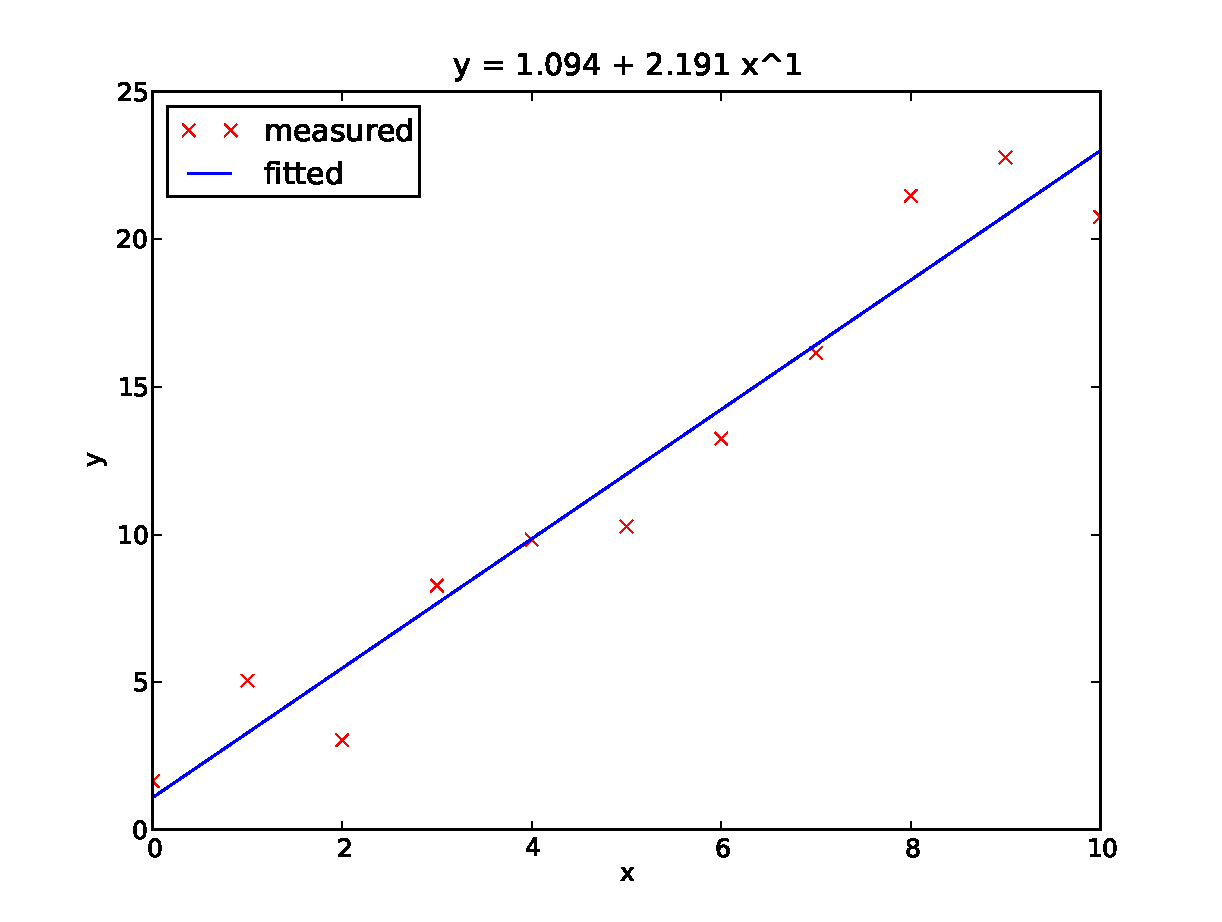
\includegraphics[width=0.5\columnwidth]{polyfit-n1}\hfill
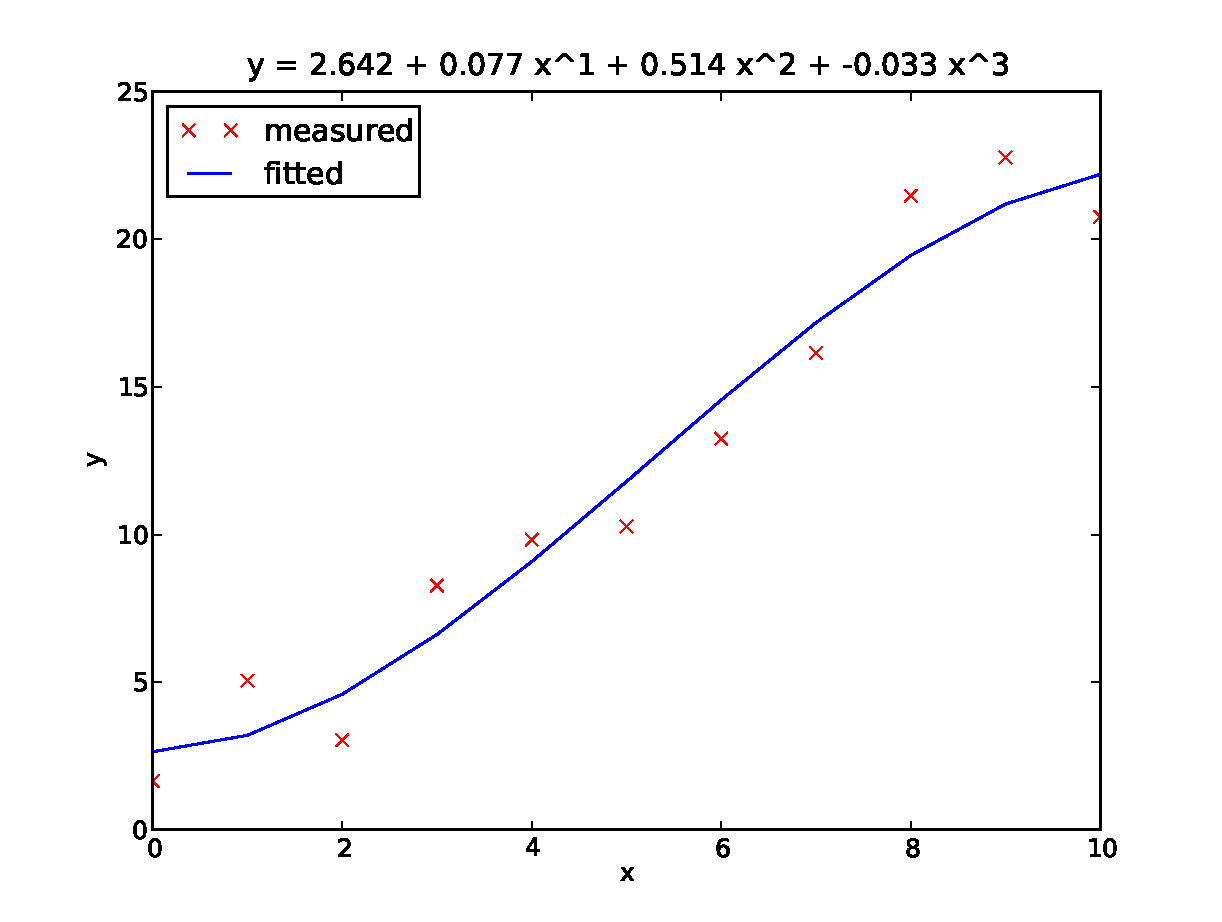
\includegraphics[width=0.5\columnwidth]{polyfit-n3}%
\caption{Polynomial fit for noisified synthetic data using first order (left) and third order (right) polynomials.}%
\label{fig:polyfit}%
\end{figure}

In the following we continue with C++ but all could be done with Python.

%%%%%%%%%%%%%%%%%%%%%%%%%%%%%%%%%%%%%%%%%%%%%%%%%%%%%%%%%%%%%%%%%%%%%%%%%%%
\section{General concepts using 1D DC resistivity inversion}\label{sec:dc1d}
{\em See cpp/py files in the directory \file{doc/tutorial/code/dc1d}.}
\subsection{Smooth inversion}\label{sec:dc1dsmooth}
{\em Example file \file{dc1dsmooth.cpp}.}\\
Included into the GIMLi library are several electromagnetic 1d forward operators.
For direct current resistivity there is a semi-analytical solution using infinite sums that are approximated by Ghosh filters. 
The resulting function calculates the apparent resistivity of any array for a given resistivity and thickness vector.
There are two main parameterization types:
\begin{itemize}
	\item a fixed parameterization where only the parameters are varied 
	\item a variable parameterization where parameters and geometry is varied
\end{itemize}

Although for 1d problems the latter is the typical one (resistivity and thickness), we start with the first since it is more general for 2d/3d problems and actually easier.
Accordingly, in the file dc1dmodelling.h/cpp two classes called \cw{DC1dRhoModelling} and \cw{DC1dBlockModelling} are defined.
For the first we first define a thickness vector and create a mesh using the function \cw{createMesh1d}.
The the forward operator is initialized with the data.

\begin{lstlisting}[language=C++]
    RMatrix abmnr; loadMatrixCol( abmnr, dataFile ); //! read data
    RVector ab2 = abmnr[0], mn2 = abmnr[1], rhoa = abmnr[2]; //! 3 columns
    RVector thk( nlay-1, max(ab2) / 2 / ( nlay - 1 ) ); //! const. thickn.
    DC1dRhoModelling f( thk, ab2, mn2 ); //! initialise forward operator
\end{lstlisting}

Note that the mesh generation can also be done automatically using another constructor.
However most applications will read or create a mesh from in application and pass it.

By default, the transformations for data and model are identity transformations.
We initialise two logarithmic transformations for the resistivity and the apparent resistivity by 
\begin{lstlisting}[language=C++]
    RTransLog transRho;
    RTransLog transRhoa;
\end{lstlisting}

Alternatively, we could set lower/upper bounds for the resistivity using
\begin{lstlisting}[language=C++]
    RTransLogLU transRho( lowerbound, upperbound);
\end{lstlisting}
Appendix \ref{app:trans} gives an overview on available transformation functions.

Next, the inversion is initialized and a few options are set
\begin{lstlisting}[language=C++]
    RInversion inv( data.rhoa(), f, verbose );
    inv.setTransData( transRhoa );           //! data transform
    inv.setTransModel( transRho );           //! model transform
    inv.setRelativeError( errPerc / 100.0 ); //! constant relative error
\end{lstlisting}

A starting model of constant values (median apparent resistivity) is defined
\begin{lstlisting}[language=C++]
    RVector model( nlay, median( data.rhoa() ) ); //! constant vector
    inv.setModel( model );                        //! starting model
\end{lstlisting}

Finally, the inversion is called and the model is retrieved using \lstinline|model = inv.run();|

A very important parameter is the regularization parameter $\lambda$ that controls the strength of the smoothness constraints (which are the default constraint for any 1d/2d/3d mesh).
Whereas $w^c$ and $w^m$ are dimensionless and 1 by default, $\lambda$ has, after eq. (\ref{eq:min}), the reciprocal and squared unit of $m$ and can thus have completely different values for different problems\footnote{The regularization parameter has therefore to be treated logarithmically.}.
However, since often the logarithmic transform is used, the default value of $\lambda=20$ is often a first guess.
Other values are set by
\begin{lstlisting}
    inv.setLambda( lambda ); //! set regularization parameter
\end{lstlisting}

In order to optimise $\lambda$, the L-curve \citep{guentherruecker06,guentherdiss} can be applied to find a trade-off between data fit and model roughness by setting \lstinline|inv.setOptimizeLambda(true);|.
For synthetic data or field data with well-known errors we can also call \lstinline|model = inv.runChi1();|, which varies $\lambda$ from the starting value such that the data are fitted within noise ($\chi^2=1$).
We created a synthetic model with resistivities of 100(soil)-500(unsaturated)-20(saturated)-1000(bedrock) $\Omega$m and thicknesses of 0.5, 3.5 and 6 meters.
A Schlumberger sounding with AB/2 spacings from 1.0 to 100\,m was simulated and 3\% noise were added.
Data format of the file \file{sond1-100.dat} is the unified data format\footnote{See \url{www.resistivity.net?unidata} for a description.}.

\begin{figure}[htbp]
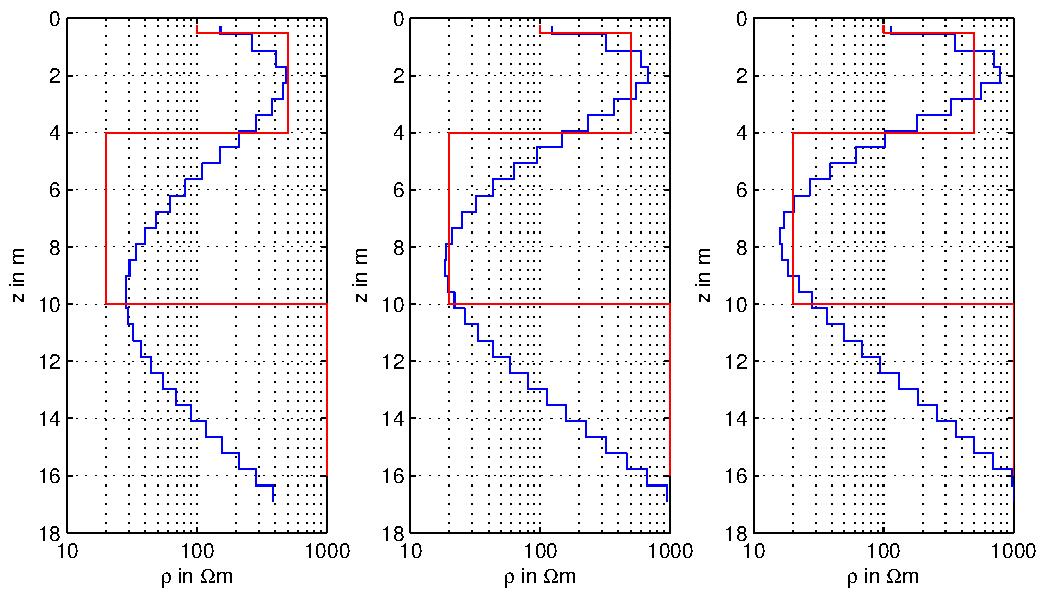
\includegraphics[width=\textwidth]{sond1-100-3lambdas}\\[-3ex]
~~~a\hfill ~~~b \hfill ~~~c \hfill ~
\caption{Smooth 1d resistivity inversion results for a) $\lambda=200\Rightarrow \chi^2=11.1$/rrms=10.1\%, b) $\lambda=20\Rightarrow \chi^2=1.2$/rrms=3.3\%, and c) $\lambda=2\Rightarrow \chi^2=0.6$/rrms=2.4\%, red-synthetic model, blue-estimated model}\label{fig:dc1d-3lambda}
\end{figure}

Figure~\ref{fig:dc1d-3lambda} shows the inversion result for the three different regularization parameters 300, 30 and 3.
Whereas the first is over-smoothed, the other are much closer at the reality.
The rightmost figure over-fits the data ($\chi^2=0.3<1$) but is still acceptable.
The L-curve method yields a value of $\lambda=2.7$, which is too low.
However, if we apply the $\chi^2$-optimization we obtain a value of $\lambda=15.2$ and with it the data are neither over- nor under-fitted.

%%%%%%%%%%%%%%%%%%%%%%%%%%%%%%%%%%%%%%%%%%%%%%%%%%%%%%%%%%%%%%%%%%%%%%%%%%%
\subsection{Block inversion}\label{sec:dc1dblock}
{\em Example file \file{dc1dblock.cpp} in the directory \file{doc/tutorial/code/dc1d}.}\\
Alternatively, we might invert for a block model with unknown layer thickness and resistivity.
We change the mesh generation accordingly and use the forward operator \lstinline|DC1dModelling|:
\begin{lstlisting}[language=C++]
    DC1dModelling f( nlay, ab2, mn2 );
\end{lstlisting}

\lstinline|createMesh1DBlock| creates a block model with two regions\footnote{With a second argument \lstinline|createMesh1DBlock| can create a block model with thickness and several parameters for a multi-parameter block inversion.}.
Region 0 contains the thickness vector and region 1 contains the resistivity vector.
There is a region manager as a part of the forward modelling class that administrates the regions.
We first define different transformation functions for thickness and resistivity and associate it to the individual regions.
\begin{lstlisting}[language=C++]
    RTransLog transThk;
    RTransLogLU transRho( lbound, ubound );
    RTransLog transRhoa;
    f.region( 0 )->setTransModel( transThk );
    f.region( 1 )->setTransModel( transRho );
\end{lstlisting}

For block discretisations, the starting model can have a great influence on the results.
We choose the median of the apparent resistivities and a constant thickness derived from the current spread as starting values.
\begin{lstlisting}[language=C++]
    double paraDepth = max( ab2 ) / 3;		
    f.region( 0 )->setStartValue( paraDepth / nlay / 2.0 );
    f.region( 1 )->setStartValue( median( rhoa ) );
\end{lstlisting}

For block inversion a scheme after \cite{marquardt}, i.e. a local damping of the changing without interaction of the model parameters and a decreasing regularization strength is favourable.
\begin{lstlisting}[language=C++]
    inv.setMarquardtScheme( 0.9 ); //! local damping with decreasing lambda
\end{lstlisting}

The latter could also be achieved by \begin{enumerate}
	\item setting the constraint type to zero (damping) by \lstinline|inv.setConstraintType(0)|
	\item switching to local regularization by \lstinline|inv.setLocalRecularization(true)|
	\item defining the lambda decreasing factor by \lstinline|inv.setLambdaDecrease(0.9)|
\end{enumerate}

%The choice of appropriate regularization parameters is somewhat more complicated since the result strongly depends on the starting model and the preceding models \citep{guentherdiss}.
%The latter can be done by \lstinline|inv.setLambdaDecrease( factor );|

With the default regularization strength $\lambda=20$ we obtain a data fit slightly below the error estimate.
The model (Fig.~\ref{fig:dc1dblock-resres}a) clearly shows the four layers (blue) close to the synthetic model (red).
%Some parameters are overestimated and some are underestimated.

\begin{figure}[htbp]
\centering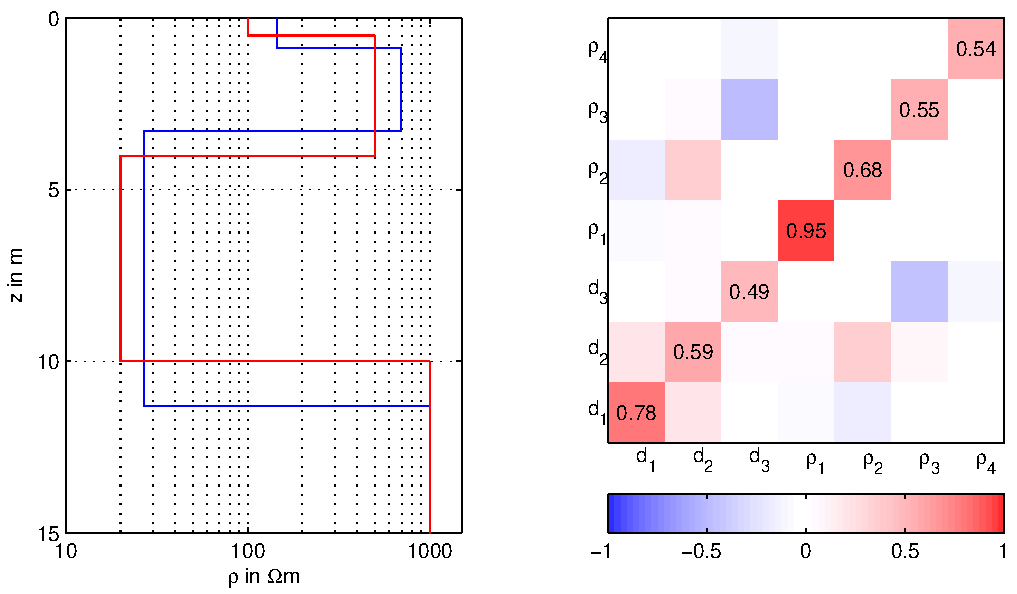
\includegraphics[width=0.7\textwidth]{dc1dblock-resres}\\[-3ex]
~\hfill a\hfill ~ \hfill ~~~~~b \hfill ~ \hfill ~ \hfill ~
\caption{a) Block 1d resistivity inversion result (red-synthetic model, blue-estimated model)) and b) resolution matrix}\label{fig:dc1dblock-resres}
\end{figure}

%%%%%%%%%%%%%%%%%%%%%%%%%%%%%%%%%%%%%%%%%%%%%%%%%%%%%%%%%%%%%%%%%%%%%%%%%%%
\subsection{Resolution analysis}\label{sec:dc1dresolution}
One may now be interested in the resolution properties of the individual model parameters.
The resolution matrix $\R^M$ defines the projection of the real model onto the estimated model:
\begin{equation}
	\m^{est} = \R^M \m^{true} + (\I - \R^M) \m^R + \S^\dagger\D\n\quad,
\end{equation}
\citep{guentherdiss} where $\S^\dagger\D\n$ represents the generalised inverse applied to the noise.
Note that $\m^R$ changes to $\m^k$ for local regularization schemes \citep{friedel03}.

\citet{guentherdiss} also showed that the model cell resolution (discrete point spread function) can be computed by solving an inverse sub-problem with the corresponding sensitivity distribution instead of the data misfit.
This is implemented in the inversion class by the function \lstinline|modelCellResolution( iModel )| where \lstinline|iModel| is the number of the model cell.
This approach is feasible for bigger higher-dimensional problems and avoids the computation of the whole resolution matrix.
A computation for representative model cells can thus give insight of the resolution properties of different parts of the model.

For the block model we successively compute the whole resolution matrix.
\begin{lstlisting}
    RVector resolution( nModel ); //! create single resolution vector
    RMatrix resM;                 //! create empty matrix 
    for ( size_t iModel = 0; iModel < nModel; iModel++ ) {
        resolution = inv.modelCellResolution( iModel );
        resM.push_back( resolution );  //! push back the single vector
    }
    save( resM, "resM" ); //! save resolution matrix
\end{lstlisting}

In Figure~\ref{fig:dc1dblock-resres} the model resolution matrix is shown and the diagonal elements are denoted.
The diagonal elements show that the resolution decreases with depth.
The first resistivity is resolved nearly perfect, whereas the other parameters show deviations from 1.
$\rho_2$ is positively connected with $d_2$, i.e. an increase of resistivity can be compensated by an increased resistivity.
For $\rho_3$ and $d_3$ the correlation is negative.
These are the well known H- and T-equivalences of thin resistors or conductors, respectively, and show the equivalence of possible models that are able to fit the data within noise.
%Similarly, we can obtain the resolution kernels also for smooth inversion.

%%%%%%%%%%%%%%%%%%%%%%%%%%%%%%%%%%%%%%%%%%%%%%%%%%%%%%%%%%%%%%%%%%%%%%%%%%%
\subsection{Structural information}\label{sec:dc1dstruct}
{\em Example file \file{dc1dsmooth-struct.cpp} in the directory \file{doc/tutorial/code/dc1d}.}\\
Assume we know the ground water table at 4\,m from a well.
Although we know nothing about the parameters, this structural information should be incorporated into the model.
We create a thickness vector of constant 0.5\,m. 
The first 8 model cells are located above the water table, so the 8th boundary contains the known information.
Therefore we set a marker different from zero (default) after creating the mesh
\begin{lstlisting}
    //! variant 1: set mesh (region) marker
    f.mesh()->boundary( 8 ).setMarker( 1 );
\end{lstlisting}
This causes the boundary between layer 8 and 9 being disregarded, the corresponding $w^c_8$ is zero and allows for arbitrary jumps in the otherwise smoothed model.
Figure~\ref{fig:dc1dsmooth-struct} shows the result, at 4\,m the resistivity jumps from a few hundreds down to almost 10.

\begin{figure}[htbp]
\centering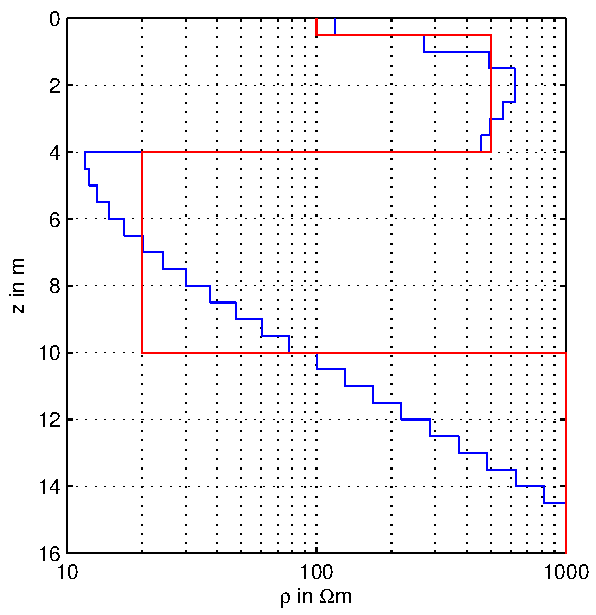
\includegraphics[width=0.45\textwidth]{sond1-100-struct.pdf}
%\\[-3ex]
%~\hfill a\hfill ~ \hfill ~~~~~b \hfill ~ \hfill ~ \hfill ~
\caption{Inversion result with the ground water table at 4\,m as structural constraint.}\label{fig:dc1dsmooth-struct}
\end{figure}

Note that we can set the weight to zero also directly, either as a property of the inversion
\begin{lstlisting}
    //! variant 2: application of a constraint weight vector to inversion
    RVector bc( inv.constraintsCount(), 1.0 );
    bc[ 6 ] = 0.0;
    inv.setCWeight( bc ); 
\end{lstlisting}
or the (only existing) region.
\begin{lstlisting}
    //! variant 3: application of a boundary control vector to region
    RVector bc( f.regionManager().constraintCount(), 1.0 );
    bc[ 7 ] = 0.0;
    f.region( 0 )->setConstraintsWeight( bc );
\end{lstlisting}
Of course, in 2d/3d inverse problems we do not set the weight by hand.
Instead, we put an additional polygon (2d) or surface (3d) with a marker $\neq 0$ into the PLC before the mesh generation.
By doing so, arbitrary boundaries can be incorporated as known boundaries.

%%%%%%%%%%%%%%%%%%%%%%%%%%%%%%%%%%%%%%%%%%
\subsection{Regions}\label{sec:dc1dregion}
{\em Example file \file{dc1dsmooth-region.cpp} in the directory \file{doc/tutorial/code/dc1d}.}\\
In the latter sections we already used regions.
A default mesh contains a region with number 0.
A block mesh contains a region 0 for the thickness values and regions counting up from 1 for the individual parameters.
Higher dimensional meshes can be created automatically by using region markers, e.g. for specifying different geological units.

In our case we can divide part above and a part below water level.
In 2d or 3d we would, similar to the constraints above, just put a region marker $\neq 0$ into the PLC and the mesh generator will automatically associate this attribute to all cells in the region.

Here we set the markers of the cells $\geq8$ to the region marker 1.
\begin{lstlisting}
    Mesh * mesh = f.mesh();
    mesh->boundary( 8 ).setMarker( 1 );
    for ( size_t i = 8; i < mesh->cellCount(); i++ ) 
        mesh->cell( i ).setMarker( 1 );
\end{lstlisting}

Now we have two regions that are decoupled automatically.
The inversion result is identical to the one in Figure~\ref{fig:dc1dsmooth-struct}.
However we can now define the properties of each region individually.
For instance, we might know the resistivities to lie between 80 and 800\,$\Omega$m above and between 10 and 100\,$\Omega$m below.
Consequently we define two transformations and apply it to the regions.
\begin{lstlisting}
    RTransLogLU transRho0( 80, 800 );
    RTransLogLU transRho1( 10, 1000 );
    f.region( 0 )->setTransModel( transRho0 );
    f.region( 1 )->setTransModel( transRho1 );
\end{lstlisting}

Additionally we might try to improve the very smooth transition between groundwater and bedrock.
We decrease the model control (strength of smoothness) in the lower region by a factor of 10.
\begin{lstlisting}
    f.region( 1 )->setModelControl( 0.1 );
\end{lstlisting}

The result is shown in Figure~\ref{fig:dc1dsmooth-region}.
The resistivity values are much better due to adding information about the valid ranges.
Furthermore the transition zone in the lower region is clear.
\begin{figure}[htbp]
\centering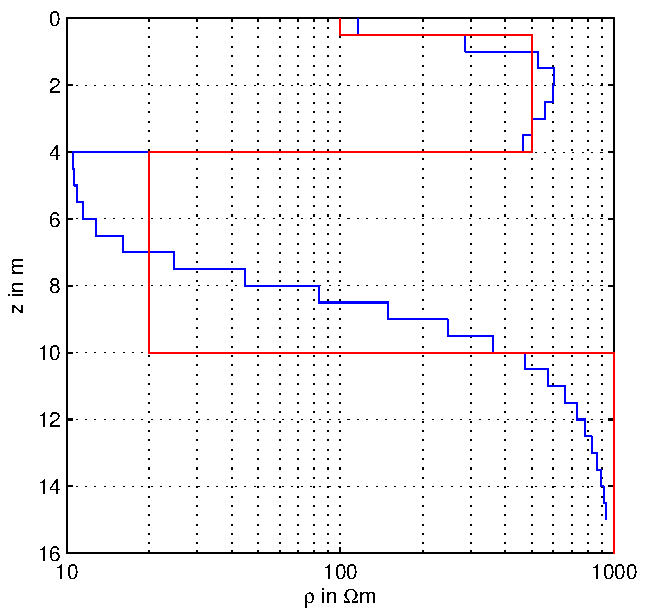
\includegraphics[width=0.45\textwidth]{sond1-100-region.pdf}
\caption{Inversion result using two regions of individual range constraint transformations and regularization strength (model control).}%
\label{fig:dc1dsmooth-region}
\end{figure}


%%%%%%%%%%%%%%%%%%%%%%%%%%%%%
\section{Enhanced techniques}\label{sec:enhanced}
\subsection{Combining different data types - MT 1d inversion}\label{sec:mt1d}
File \file{doc/tutorial/code/enhanced/mt1dinv0.cpp}\\
In magnetotelluric (MT) inversion for every period an amplitude $\rho^a$ and a phase $\phi$ is computed from the electric and magnetic registrations. The file \file{1000\_100\_1000\_n5\_1.dat} contains a synthetic three layer case of 1000$\Omega$m-100$\Omega$m-1000$\Omega$m with 5\,\% Gaussian noise on the $\rho^a$ and 1 degree on the phases.
The three columns $T$, $\rho^a$ and $\phi$ are read extracted as vectors by
\begin{lstlisting}
    RMatrix TRP; //! real matrix with period(T), resistivity(R) & phase(P)
    loadMatrixCol( TRP, dataFileName ); //! read column-based file
    size_t nP = TRP.rows(); //! number of data
    RVector T( TRP[0] ), rhoa( TRP[1] ), phi( TRP[2] ); //! columns
\end{lstlisting}
It is based on the forward operator \lstinline|MT1dModelling| in \file{src/em1dmodelling.h/cpp}, giving back a vector that consists of the amplitudes and phases for each period. 
Of course both have completely different valid ranges. 
The phases a linearly related between 0 and $\pi/2$, whereas the amplitudes are usually treated logarithmically.
On the (1d block) model side, thickness and apparent resistivity use log or logLU transforms as done for DC resistivity.
\begin{lstlisting}
    /*! Model transformations: log for resistivity and thickness */
    RTransLog transThk;
    RTransLogLU transRho( lbound, ubound );
    /*! Data transformations: log apparent resistivity, linear phases */
    RTransLog transRhoa;
    RTrans transPhi;
\end{lstlisting}
Since amplitudes and phases are combined in one vector, we create a cumulative transformation of the two by specifying their lengths. 
Similarly, the assumed relative error of the $\rho^a$ and $\phi$ are combined using a cat command.
\begin{lstlisting}
    CumulativeTrans< RVector > transData; //! combination of two trans
    transData.push_back( transRhoa, nP ); //! append rhoa trans (length nP)
    transData.push_back( transPhi, nP );  //! append phi trans
    RVector error( cat( RVector(nP,errRhoa/100), RVector(errPhase/phi) ) );
\end{lstlisting}

Similar to DC resistivity inversion, we create a 1d block mesh, initialise the forward operator and set up options for the two regions (0-thicknesses,1-resistivities).
Starting values for the $\rho_i$ and $d_i$ are computed by the mean apparent resistivity and an associated skin depth.
\begin{lstlisting}
    MT1dModelling f( T, nlay, false );
    double medrhoa = median( rhoa ); //! median apparent resistivity
    double medskindepth = sqrt( median( T ) * medrhoa ) * 503.0; //!skin d.
    f.region( 0 )->setTransModel( transThk ); //! transform
    f.region( 1 )->setTransModel( transRho );
    f.region( 0 )->setConstraintType( 0 ); //! min. length
    f.region( 1 )->setConstraintType( 0 );
    f.region( 0 )->setStartValue( medskindepth / nlay );
    f.region( 1 )->setStartValue( medrhoa );
    /*! Real valued inversion with combined rhoa/phi and forward op. */
    RInversion inv( cat( rhoa, phi ), f, verbose, dosave );
\end{lstlisting}

The rest is done as for DC resistivity block inversion.
In Figure~\ref{fig:mt1dblock-resres} the inversion result and its resolution matrix is shown.
The model is very close to the synthetic one and represents an equivalent solution.
This is also represented by the resolution matrix, where $\rho_1$, $\rho_3$ and $d_1$ are resolved almost perfectly, whereas $\rho_2$ and $d_2$ show slight deviations.
\begin{figure}[htbp]
\centering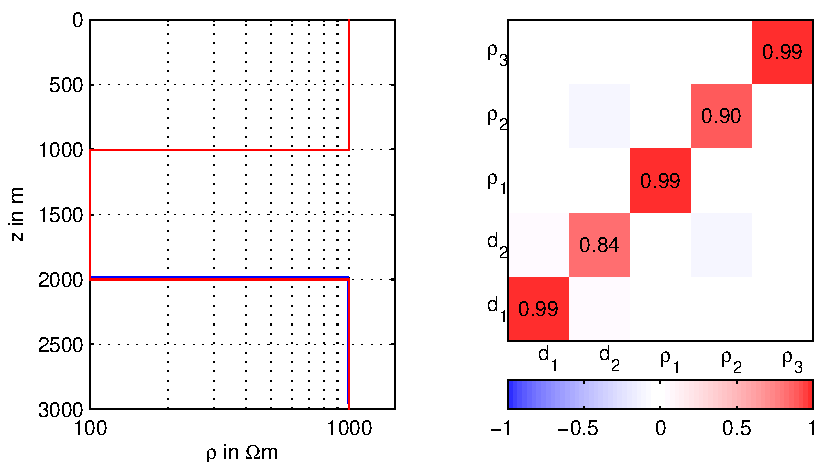
\includegraphics[width=0.7\textwidth]{mt1dblock-resres}\\[-3ex]
~\hfill a\hfill ~ \hfill ~~~~~b \hfill ~ \hfill ~ \hfill ~
\caption{a) Block 1d resistivity inversion result (red-synthetic model, blue-estimated model)) and b) resolution matrix}\label{fig:mt1dblock-resres}
\end{figure}

One can easily test the inversion only based on $\rho^a$ or $\phi$ by increasing the errors of the others by a large factor.
According to (\ref{eq:phid}) the corresponding weight goes to zero.
By skipping $\phi$ the model deviates slightly and the cell resolutions for $\rho_2$ and $d_2$ decrease to 0.9 and 0.86, respectively. If the $\rho^a$ are neglected the solution becomes obviously non-unique. Only $d_1$ is determined pretty well, the other parameters obtain cell resolutions of 0.6-0.8. Note also that for local regularization the resolution does not contain the resolution of the preceding models \citep{friedel03}.

%%%%%%%%%%%%%%%%%%%%%%%%%%%%%%%%%%%%%%%%%%%%%%%%%%%%%%%%%%%%%%%%%%
\subsection{Combining different parameter types - offsets in travel time}\label{sec:ttoffset}
Next, we consider a 2d travel-time tomographic problem.
In the library there is a forward operator called \cw{TTDijkstraModelling}, which is using a Dijkstra \citep{dijkstra} algorithm that restricts the ray paths to mesh edges. Although this is only an approximation, it is sufficiently accurate for high-quality meshes.
Assume the zero point (shot) of the traces is not exactly known. This might be due to long trigger cables, problems in the device or placing besides the profile.
Aim is to include an unknown delay for each shot position into the inversion\footnote{A similar problem is the issue of static shift in MT inversion caused by local conductivity inhomogeneity, which shifts the apparent resistivity curves.}.

First, we derive a new forward modelling class \cw{TTOffsetModelling}  from the existing \cw{TTDijkstraModelling} (abbreviated by \cw{TTMod}) since we want to use their functionality.
Additionally to the existing class we need the number of shot positions and a simple 0d/1d mesh holding the offset values for them added to the original mesh.
\begin{lstlisting}
class TTOffsetModelling : public TTMod {
public:
    TTOffsetModelling( Mesh & mesh, DataContainer & data )
      : TTMod( mesh, data ) {
        //! find occuring shots, and map them to indices starting from zero
        shots_ = unique( sort( dataContainer.get("s") ) );
        std::cout << "found " << shots_.size() << " shots." << std::endl;
        for ( size_t i = 0 ; i < shots_.size() ; i++ )
            shotMap_.insert( std::pair< int, int >( shots_[ i ], i ) );
        //! create new region containing offsets with special marker
        offsetMesh_ = createMesh1D( shots_.size() );
        for ( size_t i = 0 ; i < offsetMesh_.cellCount() ; i++ )
            offsetMesh_.cell( i ).setMarker( NEWREGION );
        regionManager().createRegion( NEWREGION, offsetMesh_ );
    }
...
\end{lstlisting}

The two functions \lstinline|response| and \lstinline|createJacobian| need to be overwritten.
However we want to expand the original functions by the changes needed.
This is straight forward for the response vector.
First part of the model is the slowness vector whose response is calculated calling the original function.

\begin{lstlisting}
    RVector TTOffsetModelling::response( const RVector & model ){
        //! extract slowness from model and call old function
        RVector slowness( model, 0, model.size() - shots_.size() );
        RVector offsets( model, model.size() - shots_.size(), model.size()); 
        RVector resp = TTMod::response( slowness ); //! normal response
        RVector shotpos = dataContainer_->get( "s" );
        for ( size_t i = 0; i < resp.size() ; i++ ){
            resp[ i ] += offsets[ shotMap_[ shotpos[ i ] ] ];
        }
        return resp;
    }
\end{lstlisting}

For the Jacobian the case is a bit more complicated.
Instead of increasing the size of the matrix a-posteriori, we use a block matrix type \lstinline|H2SparseMapMatrix| consisting of two horizontally concatenated matrices called by \lstinline|H1()| and \lstinline|H2()| \footnote{See appendix on matrices \ref{app:matrix} for existing matrix types.}.
The first is the normal way matrix holding the path lengths.
The second is a matrix with a value of 1 in the position of the shot number and 0 elsewhere.

\begin{lstlisting}
    RVector TTOffsetModelling::createJacobian( H2Matrix & jacobian, 
                                          const RVector & model ){
        //! extract slowness from model and call old function
        RVector slowness( model, 0, model.size() - shots_.size() );
        RVector offsets( model, model.size() - shots_.size(), model.size());
        TTMod::createJacobian( jacobian.H1(), slowness );
        jacobian.H2().setRows( dataContainer_->size() );
        jacobian.H2().setCols( offsets.size() );
        //! set 1 entries for the used shot
        RVector shotpos = dataContainer_->get( "s" );
        for ( size_t i = 0; i < dataContainer_->size(); i++ ) {
            jacobian.H2().setVal( i, shotMap_[ shotpos[ i ] ], 1.0 ); 
        }
    }
\end{lstlisting}

As a result the model vector holds both slowness values and the offsets, which can be sliced out of the vector for individual post-processing.

%%%%%%%%%%%%%%%%%%%%%%%
\subsection{What else?}
\begin{itemize}
	\item Full waveform TDR inversion?
	\item Gravity 2d or 3d inversion?
	\item what is enhanced?
\end{itemize}


%%%%%%%%%%%%%%%%%%%%%%%%%%%%%%%%%%%%%%%%%%%%%%%%%%%%
\section{Joint inversion}\label{sec:joint}
The term joint inversion denotes the simultaneous inversion of a number of different data types.
We can classify different types according to the relation of the associated parameters:
\begin{enumerate}
	\item Identical parameters is historical the classical joint inversion, e.g. both DC and EM aim at $\rho$.
	\item Parameters are indirectly connected by petrophysical relations, e.g. ERT and GPR both aiming at water content.
	\item Independent parameters. In this case only the structures can be linked to each other. For simple models this can involve the inversion of the geometry. For fixed models structural information is exchanged\footnote{Note that this type is formally a structurally coupled cooperative inversion.}.
\end{enumerate}

%%%%%%%%%%%%%%%%%%%%%%%%%%%%%%%%%%%%%%%%%%%%%%%%%%%%%%%%%%%%%%%%%%%%%%%%%%%
\subsection{Classical joint inversion of DC and EM soundings}\label{sec:jointdcem}
File \file{doc/tutorial/code/joint/dcem1dinv.cpp}\\
First, let us consider to jointly invert different electromagnetic methods, e.g. direct current (DC) and Frequency Domain Electromagnetic (FDEM).
For the latter we assume a two-coil system in horizontal coplanar model with 10 frequencies between 110\,Hz and 56\,kHz.
Whereas DC resistivity yields apparent resistivities, the FDEM data are expressed as ratio between secondary and primary field in per cent.

The two ready methods \lstinline|DC1dModelling| and \lstinline|FDEM1dModelling| are very easily combined since they use the same block model.
In the response function the two vectors are combined.
We create a new modelling class that derives from the base modelling class\footnote{In order to use the classes, \file{dc1dmodelling.h} and \file{em1dmodelling.h} have to be included.} and has two members of the individual classes, which must be initialized in the constructor.
Alternatively we could derive from one of the two classes and use only a member of the other.

\begin{lstlisting}[language=C++,morekeywords={RVector,RMatrix}]
class DCEM1dModelling : public ModellingBase {
public:
    DCEM1dModelling( size_t nlay, RVector & ab2, RVector & mn2, 
                     RVector & freq, double coilspacing, bool verbose ) : 
    	ModellingBase( verbose ), // base constructor
    	fDC_( nlay, ab2, mn2, verbose ), // FDEM constructor
    	fEM_( nlay, freq, coilspacing, verbose ) { // DC constructor 
          setMesh( createMesh1DBlock( nlay ) ); // create mesh
    }
    RVector response( const RVector & model ){ // paste together responses
        return cat( fDC_.response( model ), fEM_.response( model ) ); 
    }
protected:
    DC1dModelling fDC_;
    FDEM1dModelling fEM_;
};
\end{lstlisting}

In the response function both response functions are called and combined using the cat command.
We set the usual transformation (log for apparent resistivity and logLU for the resistivity) and inversion (Marquardt scheme) options as above.
In case of identical responses (e.g. apparent resistivities) this would be the whole thing.
Here we have to care about the different data types (cf. section \ref{sec:mt1d}), i.e. always positive, log-distributed $\rho_a$ from DC and possibly negative, linearly distributed, relative magnetic fields.
The transformations are again combined using \lstinline|CumulativeTrans|
\begin{lstlisting}[language=C++,morekeywords={RVector,RMatrix}]
    RTransLog transRhoa;
    RTrans transEM;
    CumulativeTrans< RVector > transData;
    transData.push_back( transRhoa, ab2.size() );
    transData.push_back( transEM, freq.size() * 2 );
\end{lstlisting}

In the code we create a synthetic model \lstinline|synthModel|, calculate the forward response and noisify it by given noise levels.

\begin{lstlisting}[language=C++,morekeywords={RVector,RMatrix}]
    /*! compute synthetic model (created before) by calling f */
    RVector synthData( f( synthModel ) );   
    /*! error models: relative percentage for DC, absolute for EM */
    RVector errorDC = synthData( 0, ab2.size() ) * errDC / 100.0;
    RVector errorEM( freq.size() * 2, errEM );
    RVector errorAbs( cat( errorDC, errorEM ) );    
    /*! noisify synthetic data using the determined error model */
    RVector rand( synthData.size() );
    randn( rand );
    synthData = synthData + rand * errorAbs;
\end{lstlisting}

The inversion is converging to a $\chi^2$ value of about 1, i.e. we fit the data within error bounds.
Finally a resolution analysis is done to determine how well the individual parameters (2 thickness and 3 resistivitiy values) are determined.
We can compare it with single inversions by drastically increasing the error level for one of the methods by a factor of 10.
Table \ref{tab:dcemresolution} shows the resulting diagonal values of the resolution matrix for a three-layer model.
The first layer is well resolved in all variants except the first layer resistivity for EM.
Considering the values for the other resistivities we can clearly see that EM is detecting the good conductor and DC describes the resistor as expected from the theory.

\begin{table}[h]%
\centering
\begin{tabular}{r|ccccc}
Method & $d_1$=20\,m & $d_2$=20\,m & $\rho_1$=200\,$\Omega$m & $\rho_2$=10\,$\Omega$m & $\rho_3$=50\,$\Omega$m \\ \hline
Joint inversion: & 0.98 & 0.46 & 0.98 & 0.67 & 0.57 \\
EM dominated:    & 0.97 & 0.36 & 0.71 & 0.66 & 0.20 \\
DC dominated:    & 0.96 & 0.21 & 0.97 & 0.32 & 0.62  
\end{tabular}
\caption{Resolution measures for Joint inversion and quasi-single inversions using an error model increased by a factor of 10.}\label{tab:dcemresolution}
\end{table}

%%%%%%%%%%%%%%%%%%%%%%%%%%%%%%%%%%%%%%%%%%%%%%%%%%%%%%%%%%%%%%%%%%%%%%%%%%%
\subsection{Block joint inversion of DC/MRS data}\label{sec:blockjoint}
%File \file{doc/tutorial/code/joint/dc\_mt\_block1d.cpp}\\
If the underlying parameters of the jointed inversion are independent, a combination can only be achieved via the geometry.
For the case of a block 1d discretization both methods are affected by the layer thicknesses.
%We use the same methods as before \sperre

Similar to the above example, we create a combined modelling class that is derived from one method, in this case \lstinline|MRS1DBlockModelling|.
This one is a block model (water content and thickness) variant of the magnetic resonance sounding (MRS) modelling \lstinline|MRSModelling|.
The class has a DC resistivity forward modelling and holds the number of layers \lstinline|nlay|.

The model is created in the constructor using \lstinline|createMesh1DBlock( nlay, 2 )| that is able to hold, additionally to the thickness (region 0), multiple properties, here water content (region 1) and resistivity (region 2).
From the model vector the thickness, water content (or their combination) and resistivity has to be extracted and the result of the two forward calls are combined using the cat command.
The Jacobian is by default brute force, which is quite cheap for block models.

\begin{lstlisting}[language=C++,morekeywords={RVector,RMatrix}]
class DC_MRS_BlockModelling : public MRS1dBlockModelling{
public:
    DC_MRS_BlockModelling( size_t nlay, DataContainer & data, RMatrix & KR,
                           RMatrix & KI, RVector & zvec, bool verbose ) :
        MRS1dBlockModelling( nlay, KR, KI, zvec, verbose ), nl_( nlay ) { 
            setMesh( createMesh1DBlock( nlay, 2 ) ); //two-properties
            Mesh mymesh = createMesh1DBlock( nlay ); //single block mesh
            fDC_ = new DC1dModelling( mymesh, data, nlay, verbose );
        }
    virtual ~DC_MRS_BlockModelling( ){ delete fDC_; }
    
    RVector response( const RVector & model ){
        //! extract resistivity, watercontent & thickness from model vec
        RVector thk( model, 0 , nl_ - 1 );
        RVector wcthk( model, 0 , nl_ * 2 - 1 );
        RVector res( model, nl_ * 2 - 1 , nl_ * 3 - 1 );
        return cat( MRS1dBlockModelling::response( wcthk ), 
                    fDC_->rhoa( res, thk ) );
    }
protected:
    DC1dModelling *fDC_;
    int nl_;
};
\end{lstlisting}

In order to use the class, we have to build a cumulative data transform as in subsection \ref{sec:mt1d}.
Model transformations are logarithmic to ensure positive values, additionally an upper bound of 0.4 is defined for the water content.
\begin{lstlisting}[language=C++,morekeywords={RVector,RMatrix}]
    RTrans transVolt;    // linear voltages
    RTransLog transRhoa; // logarithmic apparent resistivities
    CumulativeTrans< RVector > transData;
    transData.push_back( transVolt, errorMRS.size() );
    transData.push_back( transRhoa, dataDC.size() );
    RTransLog transRes;
    RTransLogLU transWC(0.0, 0.4);
    RTransLog transThk;
\end{lstlisting}

In order to achieve a Marquardt inversion scheme, the constraint type is set to zero for all regions:
\begin{lstlisting}
    f.regionManager().setConstraintType( 0 );
\end{lstlisting}
Appropriately, the transformations and starting values are set.
\begin{lstlisting}
    f.region( 0 )->setTransModel( transThk );
    f.region( 0 )->setStartValue( 5.1 );
    f.region( 1 )->setTransModel( transWC );
    f.region( 1 )->setStartValue( 0.1 );
    f.region( 2 )->setTransModel( transRes );
    f.region( 2 )->setStartValue( median( dataDC.rhoa() ) );
\end{lstlisting}

We use a synthetic model of three layers representing a vadoze zone ($\rho=500\Omega$m, 0.1\% water, 4m thick), a saturated zone ($\rho=100\Omega$m, 40\% water content, 10m thick) and a bedrock ($\rho=2000\Omega$m, no water).
3\,\% and 20\,nV Gaussian noise are added to the DC and MRS data, respectively.
Figure~\ref{fig:blockjoint} shows the result of the combined inversion, which is very close to the synthetic model due to the improved information content from two models.

\begin{figure}[htb]
\centering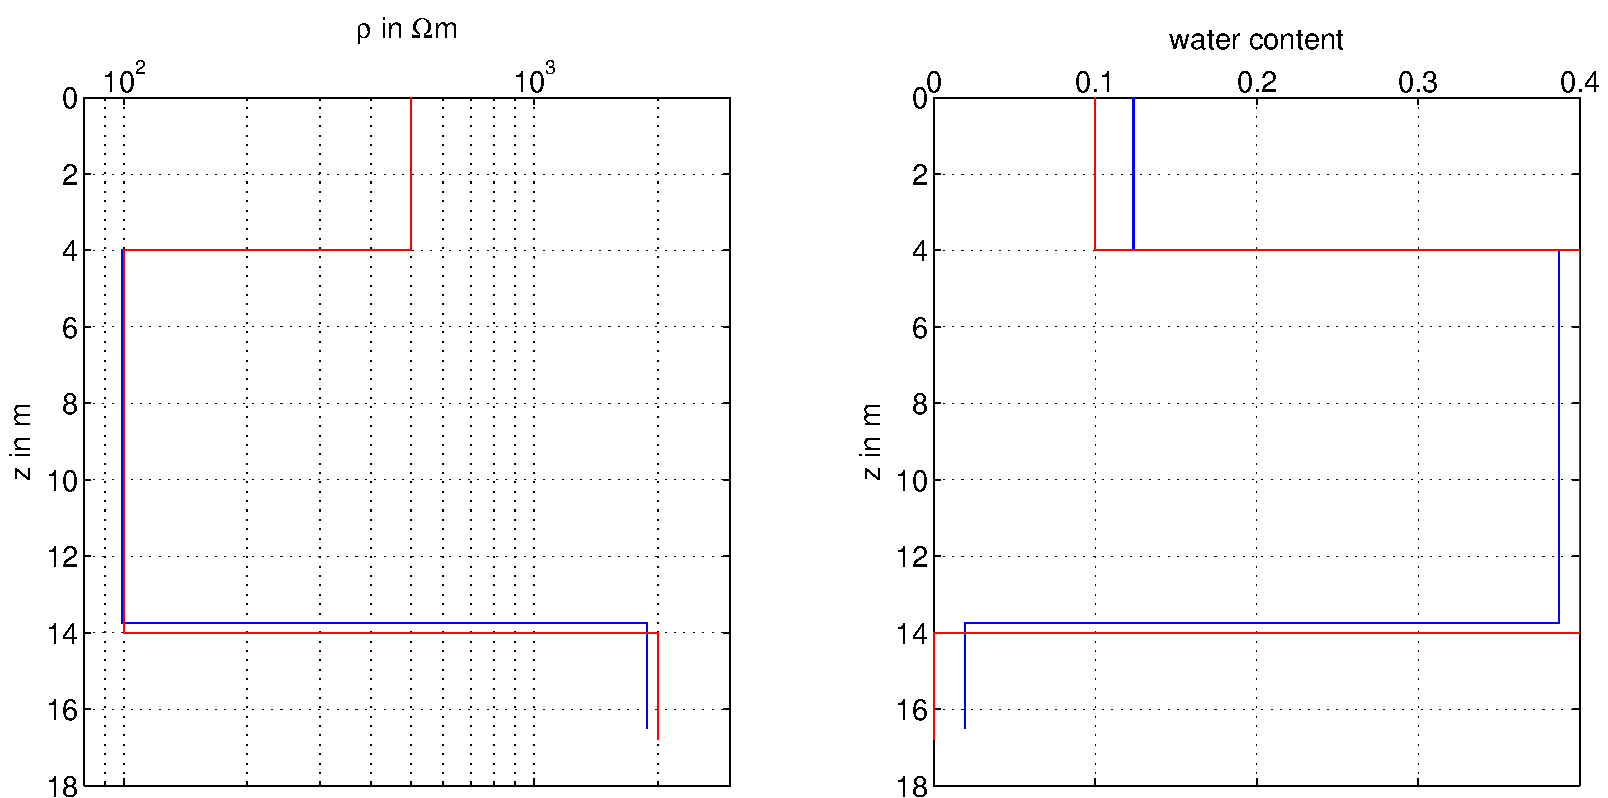
\includegraphics[width=0.9\textwidth]{dc_mrs_blockjoint}
\caption{Joint inversion result of block-coupled DC resistivity (left) and MRS (right) sounding.}\label{fig:blockjoint}
\end{figure}


%%%%%%%%%%%%%%%%%%%%%%%%%%%%%%%%%%%%%%%%%%%%%%%%%%%%%%%%%%%%%%%%%%%%%%%%%%%
\subsection{Structurally coupled cooperative inversion of DC and MRS soundings}\label{sec:structjoint}
File \file{doc/tutorial/code/joint/dc\_mrs\_joint1d.cpp}\\
In many cases it is not clear whether the model boundaries observed by different methods are identical or how many of them are existing.
Nevertheless we expect a similarity of the structure, i.e. the gradients.
On smooth model discretizations of any dimension the exchange of geometrical information can be achieved using the constraint control function \citep{guerue06nearsurface}.
Main idea is to decrease the weight for the roughness operator of one method depending on the partial derivative of the other.
A large roughness as a possible interface should enable the interface on the other side by a low weight.
There are different possible functions for doing so.
Originally, a iteratively re-weighted least squares scheme was proposed that incorporates the whole distribution.
Here we use a simple function
\begin{equation}
    w_c(r) = \frac{a}{|r|+a}+a
\end{equation}
where $w_c$ is the weight, $r$ is the roughness value and $a$ is a small quantity.
For $r\rightarrow 0$ the weight $w_c=1+a$ lies slightly above 1, for $r\rightarrow\infty$ it becomes $a$.

In this case we apply it to DC resistivity and MRS sounding for a smooth 1d model.
The latter operator is linear and thus realized by a simple matrix vector multiplication of the kernel function and the water content vector.
We initialise the two independent inversions and run one iteration step each.
In the iteration loop we calculate the function of one roughness and set it as constraint weight for the other before running another inversion step.
\begin{lstlisting}
    invMRS.setMaxIter( 1 );
    invDC.setMaxIter( 1 );
    invMRS.run(); //! init and run 1 step
    invDC.run(); //! init and run 1 step
    double a = 0.1;
    RVector cWeight( nlay - 1 );
    for ( int iter = 1; iter < maxIter; iter++ ) {
        cWeight = a / ( abs( invDC.roughness() ) + a ) + a;
        invMRS.setCWeight( cWeight );
        cWeight = a / ( abs( invMRS.roughness() ) + a ) + a;
        invDC.setCWeight( cWeight );
        invDC.oneStep();
        invMRS.oneStep();
    }
\end{lstlisting}

Figure \ref{fig:dcmrsstruct} shows the inversion result for the above mentioned three-layer case.
Without coupling (a) the transitions between the layers are quite smooth.
Much more significant jumps in both parameters occur when structural coupling is applied (b) and make the interpretation of both layer thickness and representative parameters less ambiguous.

\begin{figure}[htb]
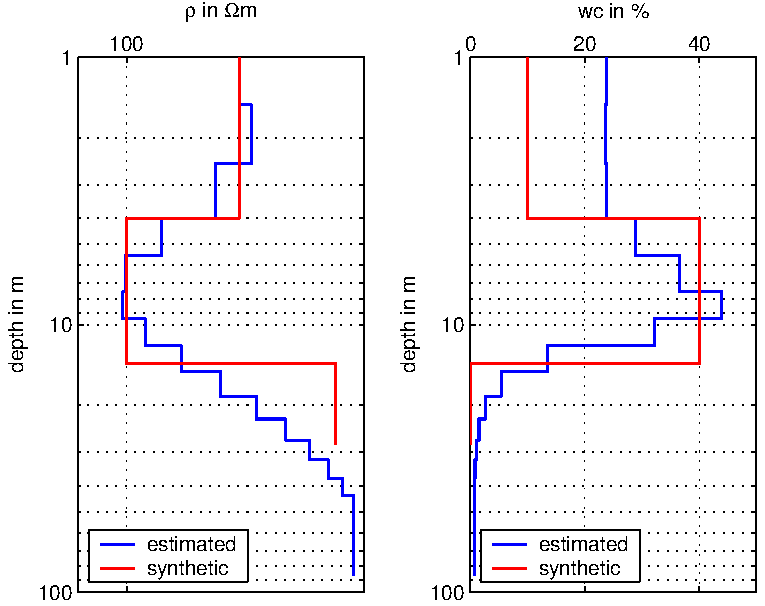
\includegraphics[width=0.5\textwidth]{DC-MRS-uncoupled}
\hfill
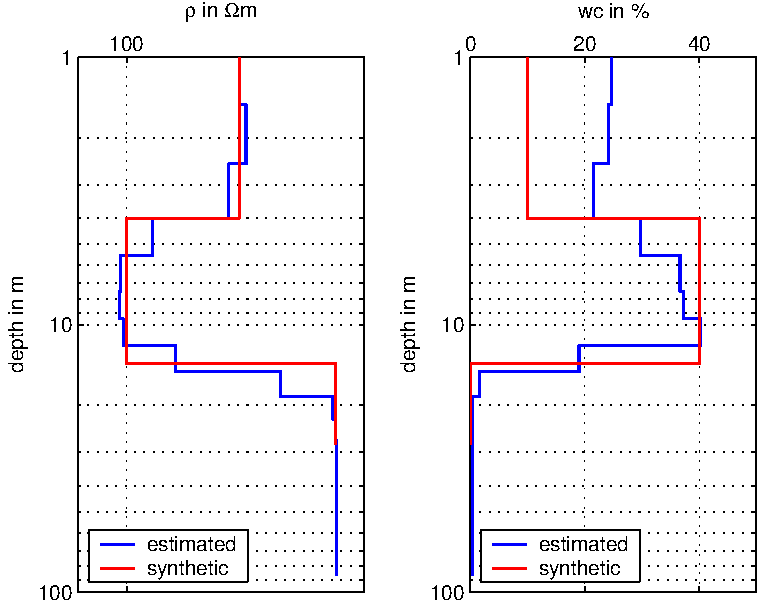
\includegraphics[width=0.5\textwidth]{DC-MRS-coupled}\\
\vskip -2ex 
a\hfill b%\\[1ex]
\caption{Synthetic model (red) and inversion results (blue) for DC (left) and MRS (right) 1D inversion without (a) and with (b) structural coupling}\label{fig:dcmrsstruct}
\end{figure} 

Of course the coupling does not have to affect the whole model.
The constraint weight vector can as well be set for an individual region such as the aquifer.
See inversion templates on how to do structural coupled inversion more easily and flexibly.

%%%%%%%%%%%%%%%%%%%%%%%%%%%%%%%%%%%%%%%%%%%%%%%%%%%%%%%%%%%%%%%%%%%%%%%%%%%
\subsection{Petrophysical joint inversion}\label{sec:petrojoint}
Target: water content in a soil column using GPR (CRIM equation) and DC (Archie equation)

\sperre{TO BE IMPLEMENTED}

\begin{figure}[htb]
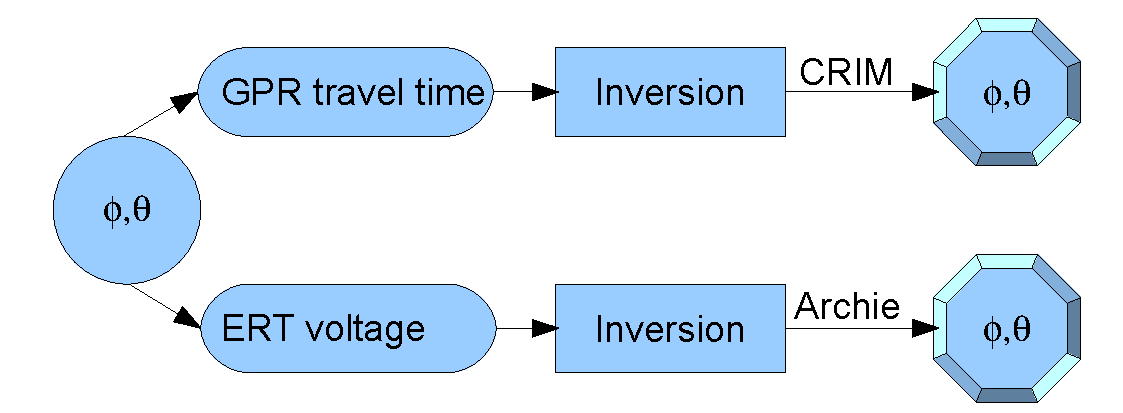
\includegraphics[width=0.5\textwidth]{petro1}
\hfill
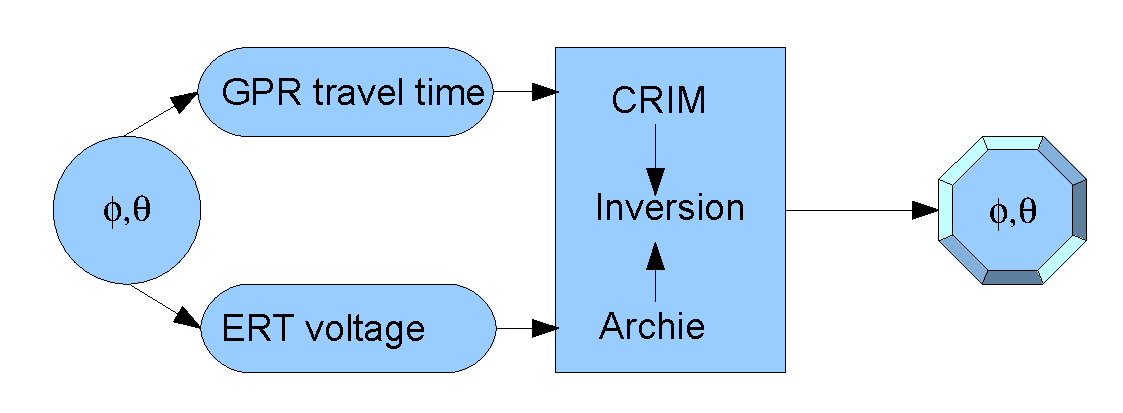
\includegraphics[width=0.5\textwidth]{petroji}\\
\vskip -8ex 
a\hfill b%\\[1ex]
\caption{Scheme for separate inversion (a) and petrophysical joint inversion (b) of GPR and ERT data to obtain an image of porosity or water content}\label{fig:petroji}
\end{figure} 


%%%%%%%%%%%%%%%%%%%%%%%%%%%%%%%%%%%%%%%%%%%%%%%%%%%%%%%%%%%%%%%%%%%%%%%%%%%
\section{Inversion templates}
There are certain tasks that go beyond a classical inversion scheme but still are method-independent.
They can be formulated more generally in order to be applied to a wider range of applications.
There are several cases
\begin{description}
\item[Roll-along inversion:] Geophysical data are often acquired along profiles. Since numerical work usually goes by $N^2$, it can be much more efficient to do the work piece-wise. However, the continuity must be ensured.
\item[Joint inversion:] As described above, the different joint inversions do not have to be programmed individually. Furthermore, more than two methods can be coupled.
\item[Time-lapse inversion:] Although there are several approaches for efficient inversion along the time axis, they are method-independent and can be formulated generally.
\end{description}

\subsection{Laterally constrained inversion}
This type is used when several 1d soundings along a line needed to be inverted together.
The forward modelling just combines the results of several soundings in a long vector.
They are individually connected to local 1d models, i.e. columns of a 2d model, which is regularized like a 2d model to achieve similarity between neighbouring models.
Accordingly, the Jacobian matrices are blocks in a block-diagonal matrix, for which an own matrix type is used.

\sperre{TO BE IMPLEMENTED}

%%%%%%%%%%%%%%%%%%%%%%%%%%%%%%%%%%%%%%%%%%%%%%%%%%%%%%%%%%%%%%%%%%%%%%%%%%%
\subsection{Roll-along inversion}
\sperre{BLA}

%%%%%%%%%%%%%%%%%%%%%%%%%%%%%%%%%%%%%%%%%%%%%%%%%%%%%%%%%%%%%%%%%%%%%%%%%%%
\subsection{Joint inversion}
Assume we have inversions invA, invB and invC, which (or parts of which) are to be coupled.

\subsubsection*{Block inversion}
Block inversion: mesh1d containing thickness and several parameters.

\sperre{TO BE IMPLEMENTED}

\subsubsection*{Structural coupling}
As described in section \ref{sec:structjoint}, the structural coupling consists mainly some preparation steps and a main iteration for the coupling that does individual runs and coupling.

Generally, there can be two possibilities for each inversion: (i) to couple the whole inversion model (as above) or (ii) to couple only one specified region.
For example, structures in an aquifer are to be imaged by cross-hole ERT and GPR. Whereas for the latter it is sufficient to restrict to the aquifer, for ERT the unsaturated zone and a clay layer must be taken into account.

For more than 2 inversions the coupling must be generalized: One can imaging a chain (or ring) or a star scheme coupling. 
Whereas in the first the inversions are coupled pair-wise, in the latter the  constraint weights are mixed. 

\begin{lstlisting}
SCCInversion SCC;
SCC.append( invA );
SCC.append( invB, regionnumber );
SCC.run(); 
\end{lstlisting}

Options: type of coupling, e.g. IRLS scheme or self-defined function. Ring or star connection. Terminating criterion.

\sperre{TO BE IMPLEMENTED}

%%%%%%%%%%%%%%%%%%%%%%%%%%%%%%%%%%%%%%%%%%%%%%%%%%%%%%%%%%%%%%%%%%%%%%%%%%%
\subsection{Time lapse inversion}\label{sec:timelapse}
\subsubsection*{Strategies}\label{sec:tlstrategies}
\subsubsection*{Example}
%DC1d infiltration??

\bibliography{gimli} 

%%%%%%%%%%%%%%%%%%%%%%%%%%%%%%%%%%%%%%%%%%%%%%%%%%%%%%%%%%%%%%%%%%%%
\begin{appendix}
\section{Inversion properties}
An inversion is a template class of the underlying data vector Vec and the matrix type Mat.
It is initialised with one of the following constructors:
\begin{lstlisting}
//! very simple and empty inversion
Inversion( bool verbose = false, bool dosave = false ) 
//! Usual inversion constructor with data and FOP
Inversion( Vec data, ModellingBase & forward, bool verbose, dosave)
//! Complete constructor including transformations
Inversion( Vec data, ModellingBase & forward, 
    Trans & transData, Trans & transModel, bool verbose, bool dosave )
\end{lstlisting}
The properties are not visible itself, instead there are setter and getter functions. Setters:
\begin{lstlisting}
setRelativeError( double/Vec error);  //! set relative data error
setAbsoluteError( double/Vec error);  //! set absolute data error
setForwardOperator( ModellingBase & forward ); //! set forward operator
setTrans( transData, transModel );   //! set transformations
setTransData( transData );           //! set data transformation
setTransModel( transModel );         //! set model transformation
setLineSearch( bool isLinesearch );  //! switch line search on/off
setRobustData( bool isRobust );      //! IRLS (robust) data weighting
setBlockyModel( bool isBlocky );     //! IRLS (blocky) model constraints
setLambda( double lambda );          //! regularisation strength
setOptimizeLambda( bool optLambda ); //! L-curve optimization
setMaxIter( int maxIter );           //! define maximum iteration number
setModel( Vec model );               //! set model vector
setModelRef( Vec referenceModel );   //! set reference model vector
setCWeight( Vec cWeight );           //! set constraint control vector
setMWeight( mWeight );               //! set model control vector
\end{lstlisting}
Getter%Vec error();
\begin{lstlisting}
ModellingBase & forwardOperator();     //! forward operator
uint boundaryCount(), modelCount(), dataCount();//! # boundaries/cells/data
bool lineSearch(), blockyModel(), robustData(), optimizeLambda();//!options
double getLambda();                   //! regularisation strength
int maxIter();                        //! maximum iteration number
Vec model(), response(), roughness(); //! model/response/roughness vector
Vec cWeight(), mWeight();             //! constraint/model control vector
getPhiD(), getPhiM(), getPhi(), getChi2(); //! objective function parts
\end{lstlisting}
Run inversion and other actions
\begin{lstlisting}
Vec model = run();               //! runs the whole inversion
Vec model = oneStep();           //! runs one inversion step
Vec model = runChi1();           //! runs changing lambda such that chi^2=1
robustWeighting();               //! applies robust data weighting
constrainBlocky();               //! apply blocky model contraints
echoStatus();                    //! echo chi2/phi/phiD/phiM/iteration
Vec modelCellResolution( iRes ); //! compute a column of resolution matrix
\end{lstlisting}

\clearpage
\section{Mesh types and mesh generation}\label{app:meshes}
There are different mesh types and ways how to generate them. There is only one base mesh class holding the nodes/vertices/coordinates, cells (defined by the bounding vertices) and boundaries revealing the neighboured cells.
Every node, cell and boundary has a marker that defines the behaviour in modelling (e.g. an electrode node or boundary conditions) or inversion (e.g. the region number or a known sharp boundary).

\subsection*{0d mesh}
Zero dimension means that there are several parameters without any neighbouring relation.
Consequently 0th order constraints are used.
There is no special mesh generator, instead a 1d mesh is created and the constraint type is set to zero.
Alternatively, the forward operator is initialised without mesh and the parameter number is set by setParameterCount.
\subsection*{1d mesh}
A real 1d mesh subdivides the subsurface in vertically or horizontally aligned elements and can be created by the following functions:
\begin{lstlisting}
/*! Generate 1d mesh with nCells cells (size 1) and nCells+1 nodes */
Mesh createMesh1D( uint nCells, uint nClones = 1 );
/*! Generate simple one dimensional mesh with nodes in RVector pos */
Mesh createMesh1D( const RVector & x );
\end{lstlisting}
nClones can be used to create models for different parameters such as resistivity and phase.
Result is one mesh with two sub-meshes that are individual regions.
See section~\ref{sec:dc1dsmooth} for an example.

\subsection*{1d block model}
A 1d block model consists of (nLayers-1) thicknesses and nLayers values for a number of properties.
The thicknesses and properties are individual 1d meshes.
\begin{lstlisting}
/*! Generate 1D block model of thicknesses and properties */
Mesh createMesh1DBlock( uint nLayers, uint nProperties = 1 );
\end{lstlisting}
See section~\ref{sec:dc1dblock} for a resistivity block inversion or \ref{sec:blockjoint} for joint block inversion using two properties.

\subsection*{2d regular mesh}
A regular (FD like) 2d model consists of regularly spaced rectangles.
They can be created by the number of elements in x- or y-direction or vectors of the enclosing nodes:
\begin{lstlisting}
/*! Generate simple 2d mesh with xDim*yDim cells of size 1 */
Mesh createMesh2D( uint xDim, uint yDim );
/*! Generate simple 2d mesh from node vectors x and y */
Mesh createMesh2D( const RVector & x, const RVector & y );
\end{lstlisting}

\subsection*{2d general mesh}
Generally a 2d mesh - a regular one is just a special case - can consist of triangles or quadrangles (deformed rectangles) or a mix of it. 
They are created by mesh generators such as triangle \citep{triangle}.
Input for the mesh is a piece-wise linear complex (PLC) comprising nodes edges and region markers.
Meshing is done externally and loaded using \lstinline|Mesh.load(filename);|.

\subsection*{3d regular mesh}
A regular (FD like) 3d model consists of regularly spaced hexahedra.
They can be created by the number of elements in x/y/z-direction or vectors of the enclosing nodes:
\begin{lstlisting}
/*! Generate regular 3d mesh with xDim*yDim*zDim cells of size 1 */
Mesh createMesh3D( uint xDim, uint yDim, uint zDim );
/*! Generate regular 3d mesh from node vectors x, y and z */
Mesh createMesh3D( const RVector & x, & y, & z );
\end{lstlisting}

\subsection*{3d general mesh}
At the moment, a 3d mesh can consist of tetrahedrons or hexahedrons, but prisms or pyramids could be easily implemented.

%%%%%%%%%%%%%%%%%%%%%%%%%%%%%%%%%%%%%%%%%%%%%%%%%%%%%%%%%%%%%%%%%%%%
\clearpage
\section{Region properties and region map file}\label{app:regions}
Some properties can be set for each region individually using \lstinline|f.region(i).|
\begin{lstlisting}
setMarker( int marker );
setBackground( bool background );
setSingle( bool single );
setStartVector( const RVector & start );
setStartValue( double start );
setModelControl( double mc );
setModelControl( const RVector & mc );
setBoundaryControl( double or RVector bc );
%setZPower( double zpower );
setZWeight( double zweight );
setTransModel( Trans & tM );
setConstraintType( uint type );
setLowerBound( double lb );
setUpperBound( double ub );
\end{lstlisting}

\begin{lstlisting}
uint parameterCount(), boundaryCount(); //! parameters/boundaries
\end{lstlisting}

The region manager controls the individual regions.
It is initialised from the forward operator and interprets the mesh with its markers
\begin{lstlisting}
setMesh( const Mesh & mesh );
Region * createRegion( int marker, const Mesh & mesh ); //! create region
Region * region( int marker ); //! get an individual region by marker
uint parameterCount(), constraintCount(), boundaryCount(); //! counters
RVector createStartVector();  //! create starting model vector
RVector createModelControl(), createBoundaryControl(); //! create vectors
RVector createFlatWeight( double zPower, double minZWeight ); //! zpower
loadMap( const std::string & fname ); //! set region properties from file
\end{lstlisting}

The latter region map file simplifies the setting of region properties and is comfortable for testing different values.
It is a column file with the description of the columns in the first row after a \# sign:
\begin{verbatim}
#No start Ctype MC  zWeight Trans lBound uBound
0   100   1     1   0.2  	  log   50     1000
1   30    0     0.2 1       log   10     200
\end{verbatim}
The example represents a two layer case, e.g. an unsaturated (0) and a saturated (1) zone with different starting resistivities.
Smoothness constraints with enhanced layering is applied in the first and minimum length in the latter.
Both use a log/logLU transformation with specific upper and lower bounds.

Instead of the number, an asterisk (*) can be used to set properties for all regions.
In one region file, several blocks as above can be stated, e.g.
\begin{verbatim}
#No start Trans
*   100   log
#No lBound uBound
1   20     300
2   50     1000
\end{verbatim}
defines an equal model transformation and starting value, but different lower and upper bounds.

There are two special types of regions: background and single regions.
The background region is not part of the inversion, the values are prolongated (filled up) for the forward run.
On the contrary, the cells of a single region are held constant and treated as one parameter in inversion.
They are specified as above using the keywords \verb|background| and \verb|single|, e.g.
\begin{verbatim}
#No single
*	1
#No background
0	1 
\end{verbatim}
defines all regions as single parameter regions except number zero, which is background.

By default, regions are decoupled from each other, i.e. there are no smoothness contraints at the boundary.
However, it might be useful to have those, e.g. by constraining a region of known parameters by borehole data to the neighboring cells or just to stabilize inversion.
In this case, inter-region constraints can be defined in the region file. 
The text
\begin{verbatim}
#Inter-region
* 	*	  0.1
1   2   1
\end{verbatim}
sets weak connection between all regions, except regions 1 and 2 are normally connected.

%%%%%%%%%%%%%%%%%%%%%%%%%%%%%%%%%%%%%%%%%%%%%%%%%%%%%%%%%%%%%%%%%%%%
\clearpage
\section{Transformation functions}\label{app:trans}
For data and model parameter arbitrary transformations can be applied.
A transformation is a C++ class derived from a base class (the identity transformation), which mainly consists of four functions, each returning a vector for a given vector:
\begin{description}
\item[trans] the forward transformation function: $y(x)$
\item[invTrans] the inverse of the function: $x(y)$
\item[deriv] the derivative of the function: $y'(x)$
\item[error] the transformation of associated errors $\delta y(\delta x)$
\end{description}
The latter is defined in the base class.
The inversion as mathematical operation is done in the $y$ domain, whereas the physics is described in the $x$ domain.

Besides the presented transformations, you can define your own transformations by deriving from the base class and overwriting the first three functions.
If the inverse transformation is not known analytically, there is a class {\bf TransNewton}, in which the inverse function is obtained by Newton iteration.

However, there are a lot of already existing transformation classes that can be used or combined:

\subsection*{Basic transforms}
\begin{description}
\item[TransLinear](a,b): $y(x)=a*x+b$
\item[TransPower]($n$): $y(x)=x^n$
\item[TransExp]($x_0$,$y_0$): $y(x)=y_0\cdot e^{-x/x_0}$
\item[TransInv]: $y(x)=1/x$ (specialisation of TransPower)
\item[TransLog]: $y(x)=\log(x)$
\end{description}

\subsection*{Range transforms}
The logarithm restricts $x$ to be positive, i.e. sets a lower bound 0.
Instead of 0, a lower bound $x_l$ can be set.
By combining two logarithmic functions a lower and an upper bound can be combined.
Similar can be obtained by a cotangens function.

\begin{description}
\item[TransLog]($x_l$): $y(x)=\log(x-x_l)$
\item[TransLogLU]($x_l$,$x_u$): $y(x)=\log(x-x_l)-\log(x_u-x)$
\item[TransCotLU]($x_l$,$x_u$): $y(x)=-\cot((x-x_l)/(x_u-x)\cdot\pi)$
\end{description}

\subsection*{Combination}
Different transformations can be combined by either\\
{\bf TransNest}($y^1$,$y^2$): $y(x)=y^1(y^2(x))$\\
{\bf TransAdd}($y^1$,$y^2$): $y(x)=y^1(x)+y^2(x)$\\
Since for the latter the inverse cannot be combined by the two inverses, it is derived from transNewton.
There is a cumulative transformation CumulativeTrans, which applies a vector of transformations for different part of the model.
This meta-transformation is applied in the region technique but can also be defined for one region.
More often it is used to combine different data types, see sections \ref{sec:mt1d} and \ref{sec:jointdcem} for examples.

\subsection*{Special transformations}
Some geophysically relevant transformations have been already defined:
\begin{description}
\item[TransLogMult]($y_0$) is a {\bf TransNest} of {\bf TransLog} and {\bf TransMult}: $y(x)=y_0\log(x_0)$, e.g. for using the logarithm of the apparent resistivity ($\rho^a=G R$)
\item[TransCRIM]($\phi$,$\epsilon_m$,$\epsilon_w$): the complex refractive index model (CRIM) - derived from {\bf TransLinear}
\item[TransArchie]($\rho_w$) - Archie's equation, derived from {\bf TransPower}
\end{description}

Note that there are predefined types based on real (double) vectors beginning with an R, e.g. \lstinline|RTransLogLU| is actually \lstinline|TransLogLU< RVector >|.


\section{Vectors and Matrix types}\label{app:matrix}
\sperre

\lstinline|std::vector|

\lstinline|template< class ValueType > class Vector|

\lstinline|RVector| 

\lstinline|load/save|

complex values using Complex = \lstinline|std::complex<double>| as a vector \lstinline|CVector|

\lstinline|template < class ValueType > class Matrix|

\lstinline|RMatrix|

\lstinline|load/saveMatrixCol|

\lstinline|template< class ValueType, class IndexType > class SparseMapMatrix|

DSparseMapMatrix for double and unsigned int

modelling SparseMatrix
\end{appendix}

\end{document}
